\providecommand{\myrootdir}{..}
\documentclass[\myrootdir/main.tex]{subfiles}

\begin{document}

\chapter{Empirical Comparison Study}
\label{sec:study}
To investigate when PBE, CTS and KWS are suited to retrieve chunks from CI build logs we evaluated our implementation of those techniques on the \emph{Failing Build Log Data Set}.
This chapter describes our study design and presents the results of the study.
The analysis of the study results first focusses on each of the three techniques and later we compare them against each other.


\begin{figure}[htbp]
	\centering
	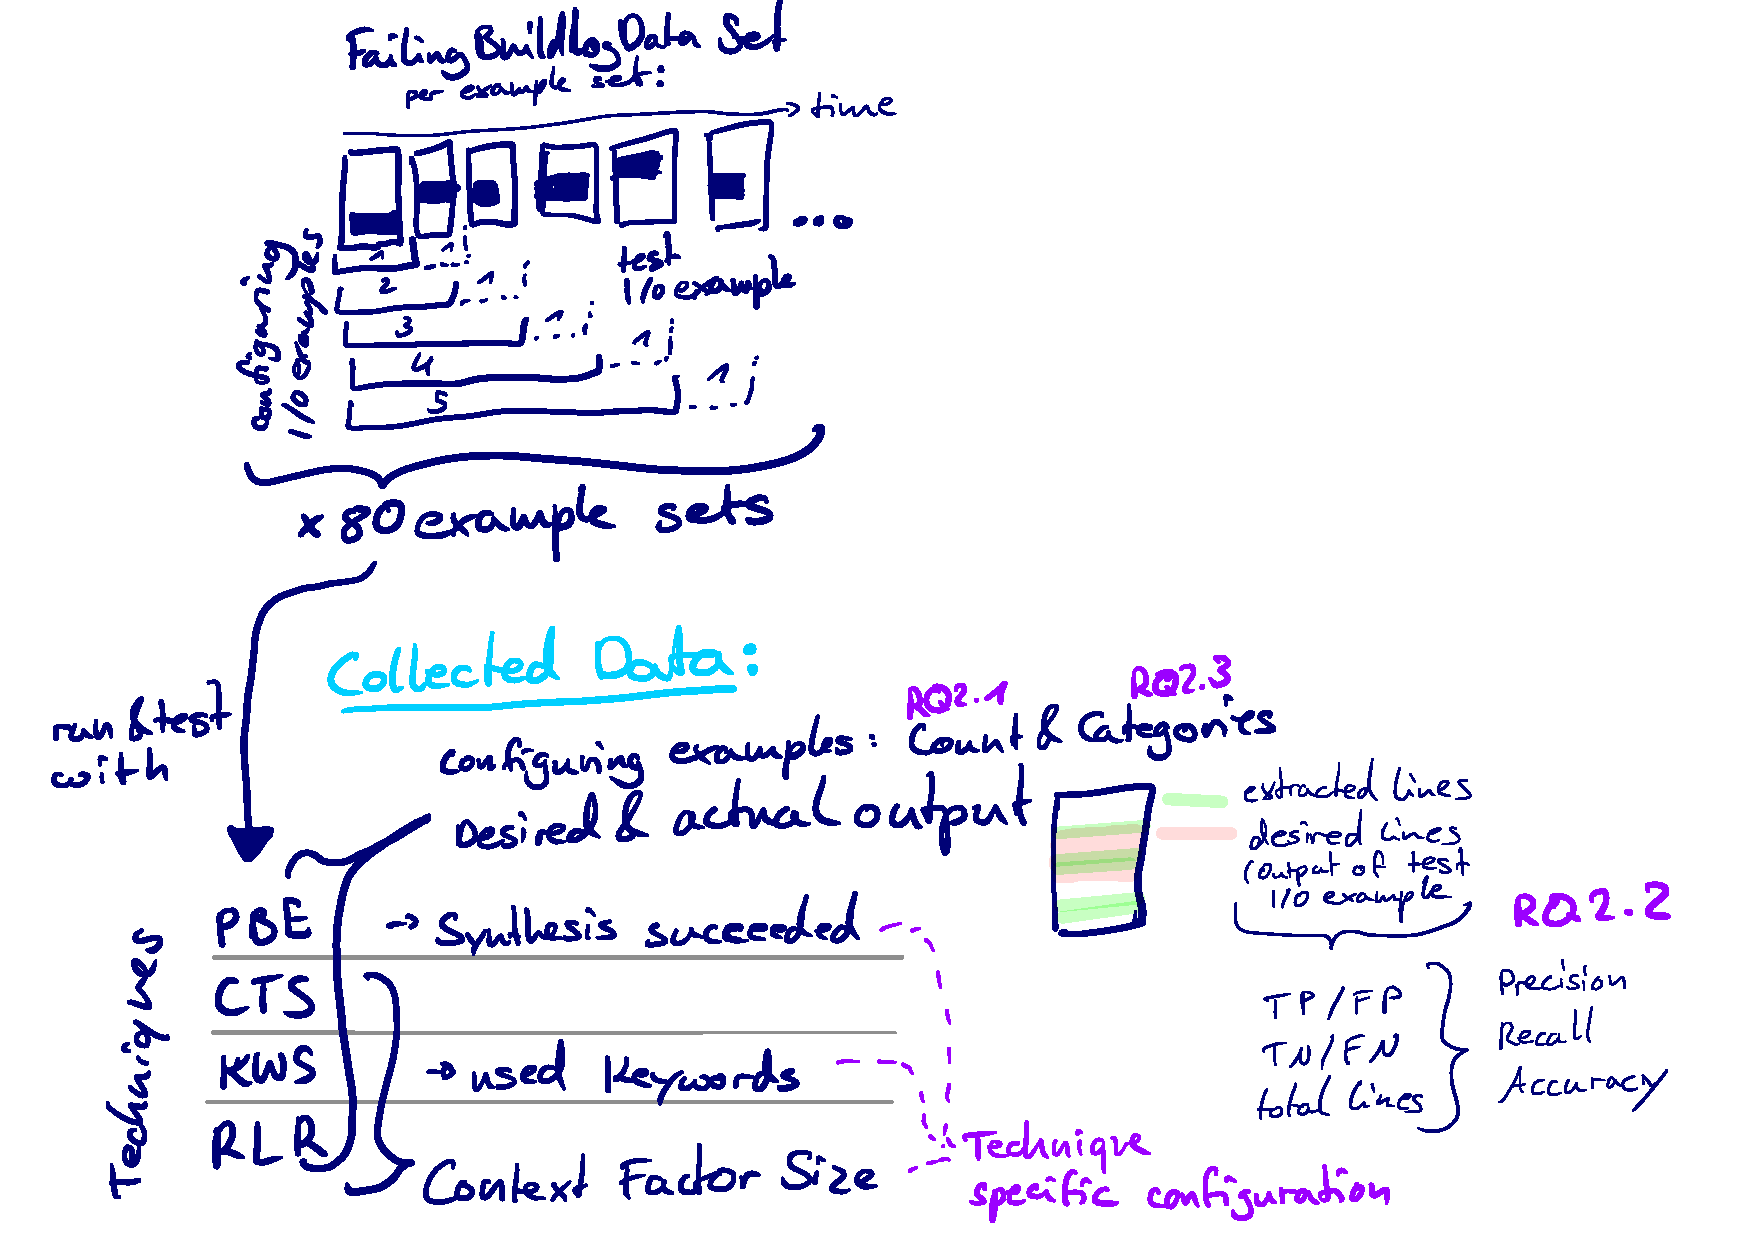
\includegraphics[width=\textwidth, clip]{img/study-design.pdf}
	\caption{Study design of our technique comparison study}
	\label{fig:study}
\end{figure}

\section{Study Design}
For the comparison study we evaluate the three chunk retrieval techniques PBE, CTS and KWS, described in Sections \ref{sec:expl-pbe},\ref{sec:expl-ts} and \ref{sec:expl-skws}.
RLR, explained in Section \ref{sec:expl-rlr}, acts as a baseline for the comparison.
We run four techniques on the example sets from the \emph{Failing Build Log Data Set}.

The examples are sorted chronologically, i.e. a technique is configured with examples from the directly preceding build logs.
For each example set and each technique, we select one to five successive I/O examples as configuration, the \emph{configuring I/O examples}, and run the chunk retrieval on the next I/O example, the \emph{test I/O example}.

For each of our evaluation runs we measure the desired vs. actual output lines of the chunk retrieval.
The desired output is given by the output of the test I/O example, which acts as the oracle for our evaluation.
From this we obtain true/false positives/negatives and calculate precision, recall and accuracy, which we use to answer \textbf{RQ2.2}.
We register the number of examples used as configuration for each run to answer \textbf{RQ2.1} and their structural categories to answer \textbf{RQ2.3}.
\todo{mention / explain retrival size facto}

%taking The Failing Build Log Data Set - run 3(4 with random) techniques with increasing example count - measuring xyz - justify choices like running chronologically / testing on 1 example / no k-fold validation - how are keywords for the search selected?

\section{Results}
This section presents the evaluation results for PBE, CTS and KWS separately.
Afterwards it compares the three techniques with each other and RLR as baseline.

% \begin{figure}[htbp]
% 	\centering
% 	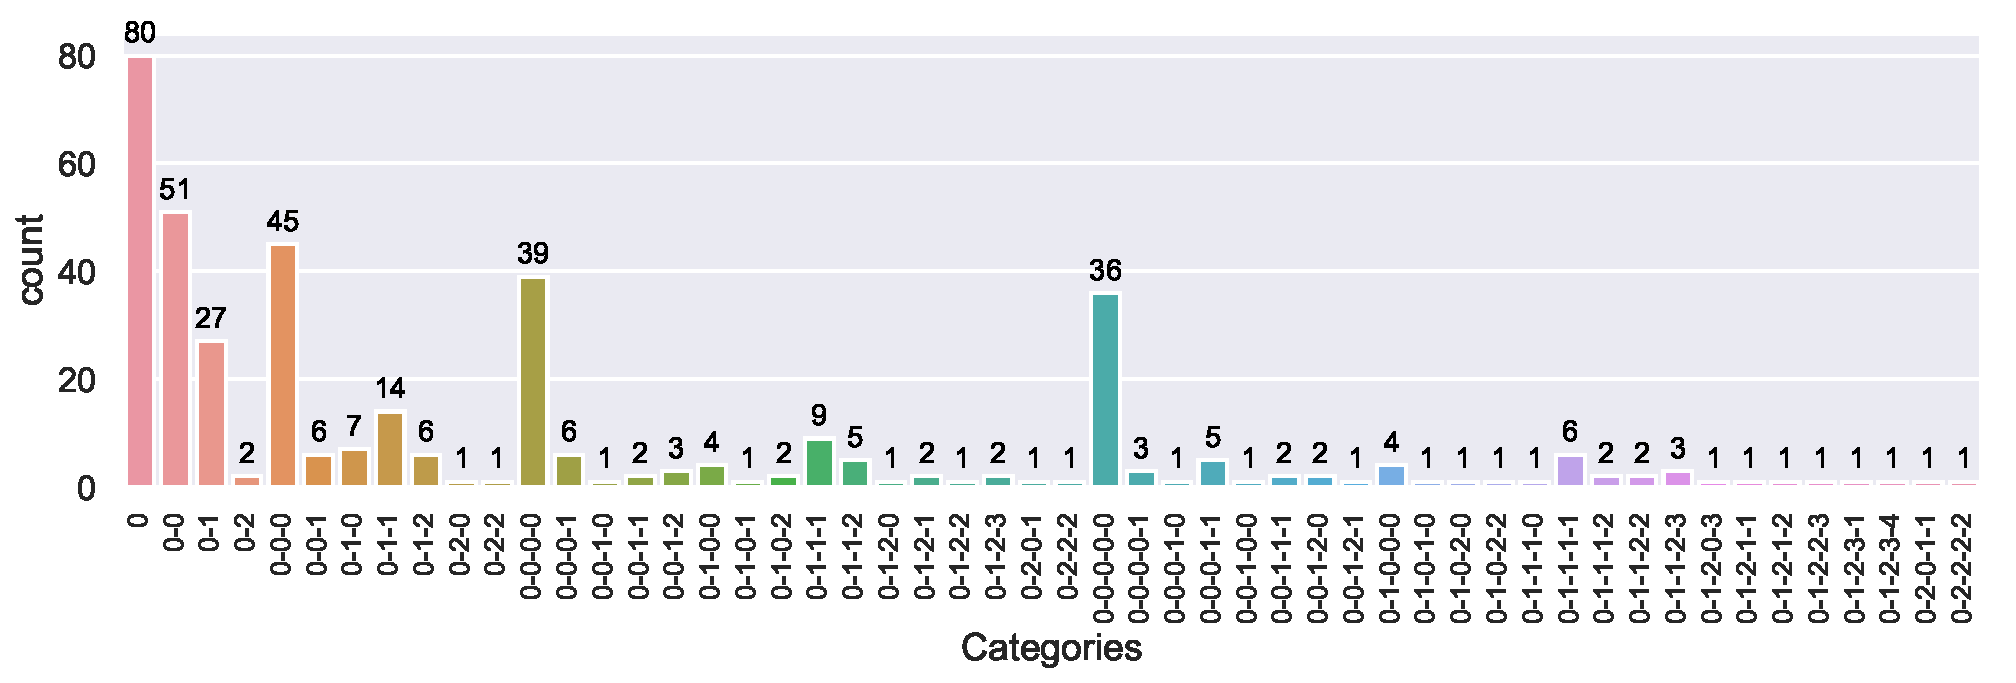
\includegraphics[width=\textwidth, clip]{img/big-study/categories-dataset.pdf}
% 	\caption{Distribution of Category Combinations in the Example Sets used for Configuration in our Study}
% 	\label{fig:categories-dataset}
% \end{figure}

% \begin{figure}[htbp]
% 	\centering
% 	\begin{minipage}{0.45\textwidth}
% 		\centering
% 		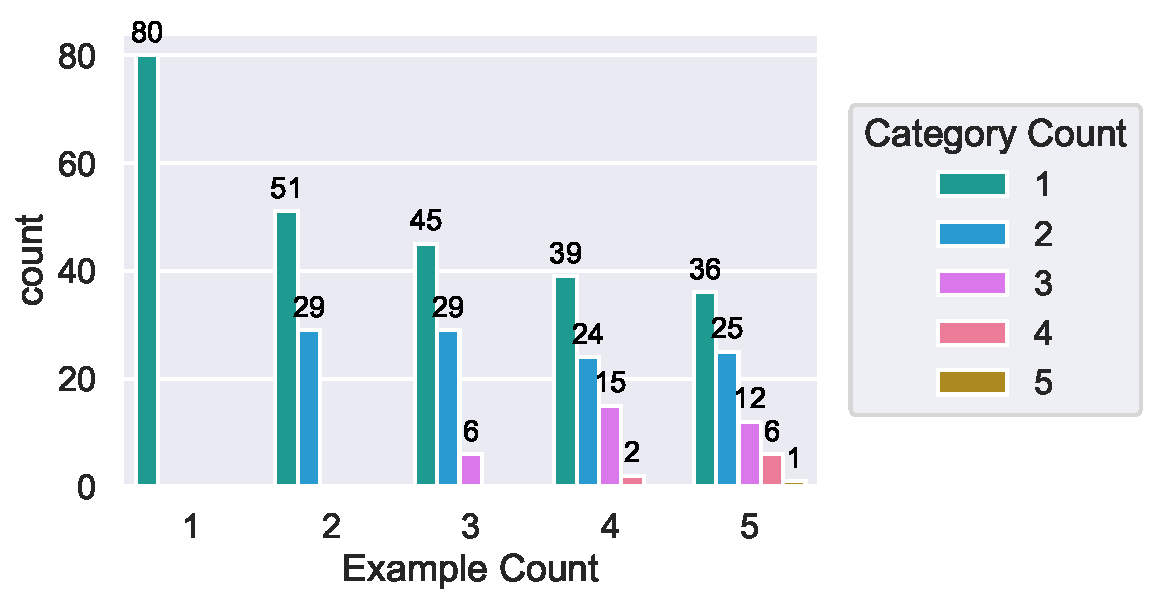
\includegraphics[width=\textwidth, clip]{img/big-study/categorycount-examplecount-dataset.pdf}
% 		\caption{Distribution of the Count of Categories within the Examples used for Configuration in our Study}
% 		\label{fig:categorycount-examplecount-dataset}
% 	\end{minipage}\hfill
% 	\begin{minipage}{0.45\textwidth}
% 		\centering
% 		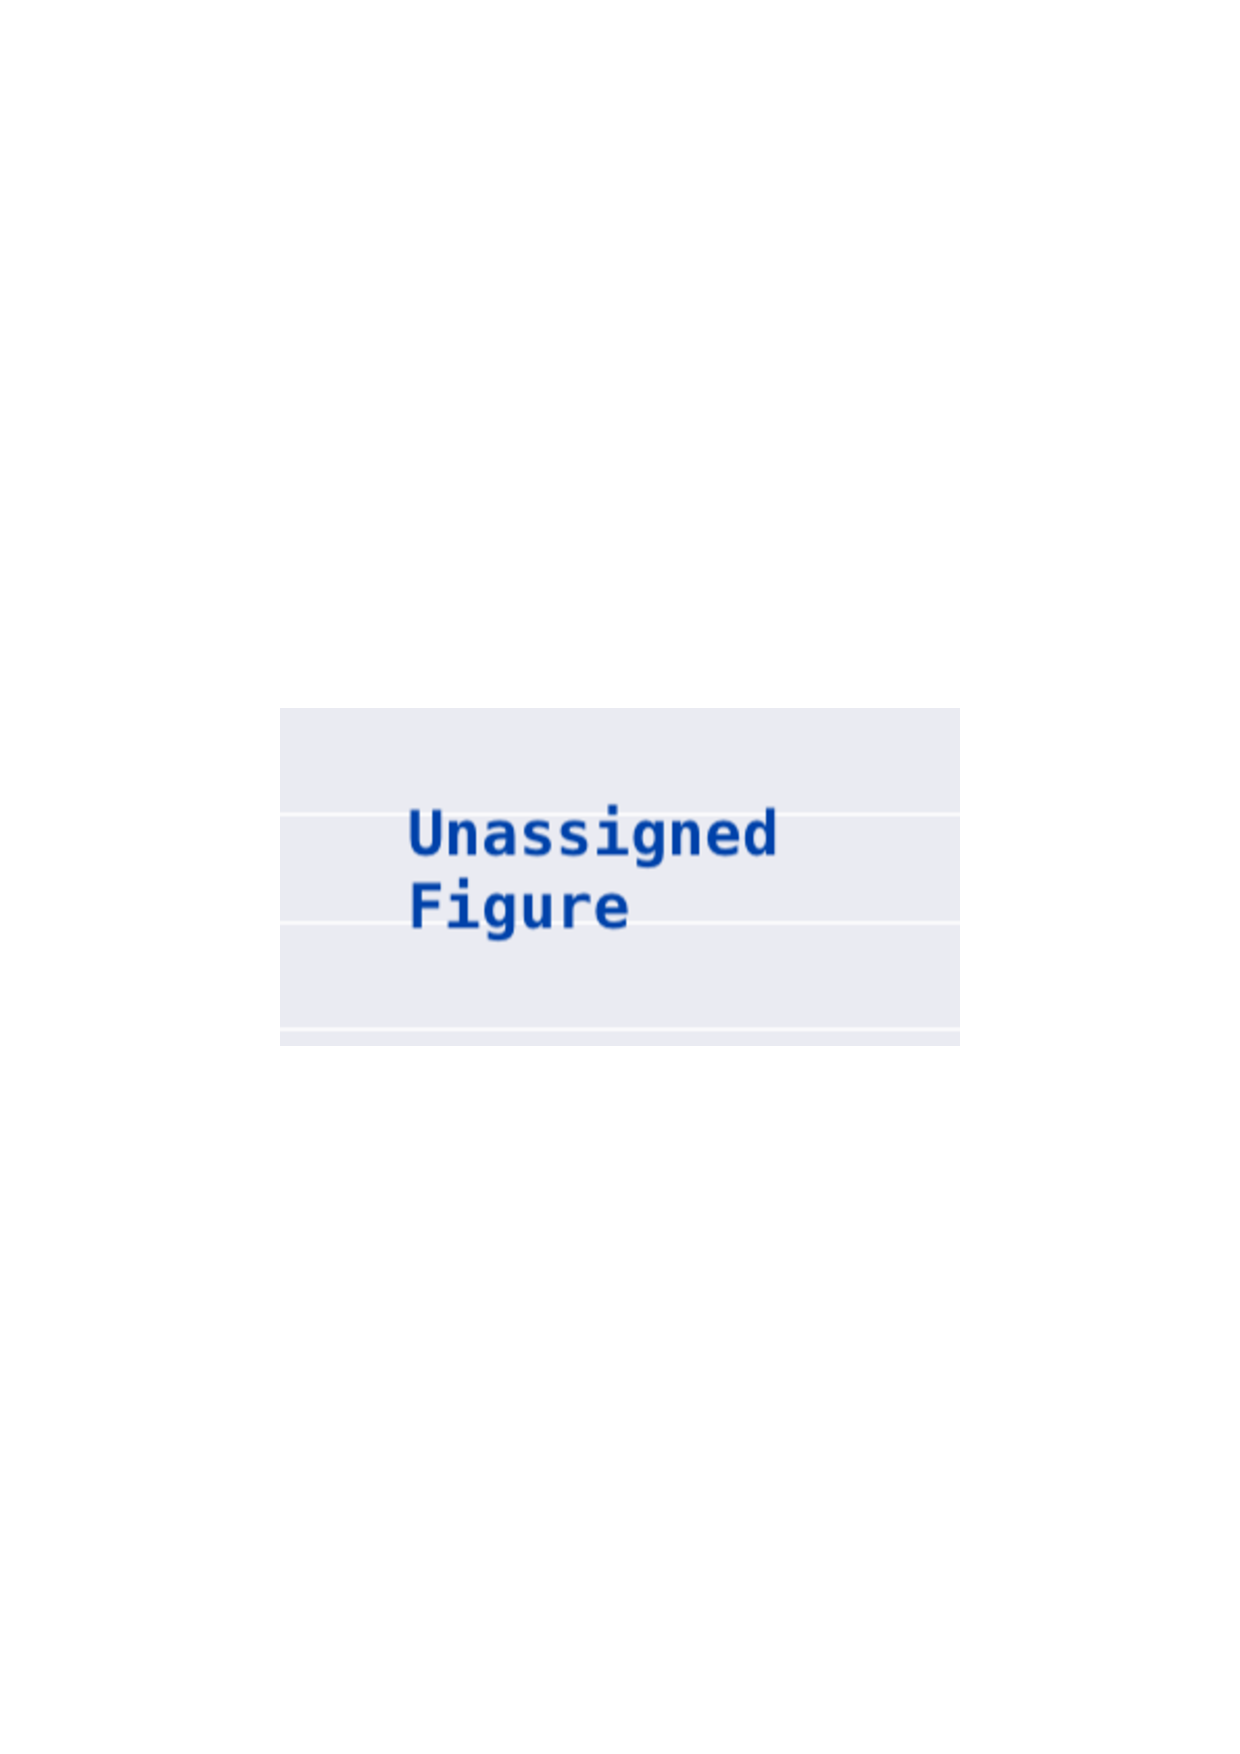
\includegraphics[width=\textwidth, clip]{img/big-study/xxx.pdf}
% 		\caption{caption}
% 		\label{fig:xxxy}
% 	\end{minipage}
% \end{figure}

% \subsection{Category Distribution in Data Set}
% Categories distributed in over data set
% - why are we looking at that?: interesting how categories are distributed for this real world example of build Failure reasons in travis ci categorization
% - Figure \ref{fig:categories-dataset} shows the distribution of categories in the configuring example sets in rou study
% - Figure \ref{fig:categorycount-examplecount-dataset} shows the category count separated by the different example count.


\begin{figure}[htbp]
	\centering
	\begin{minipage}{0.45\textwidth}
		\centering
		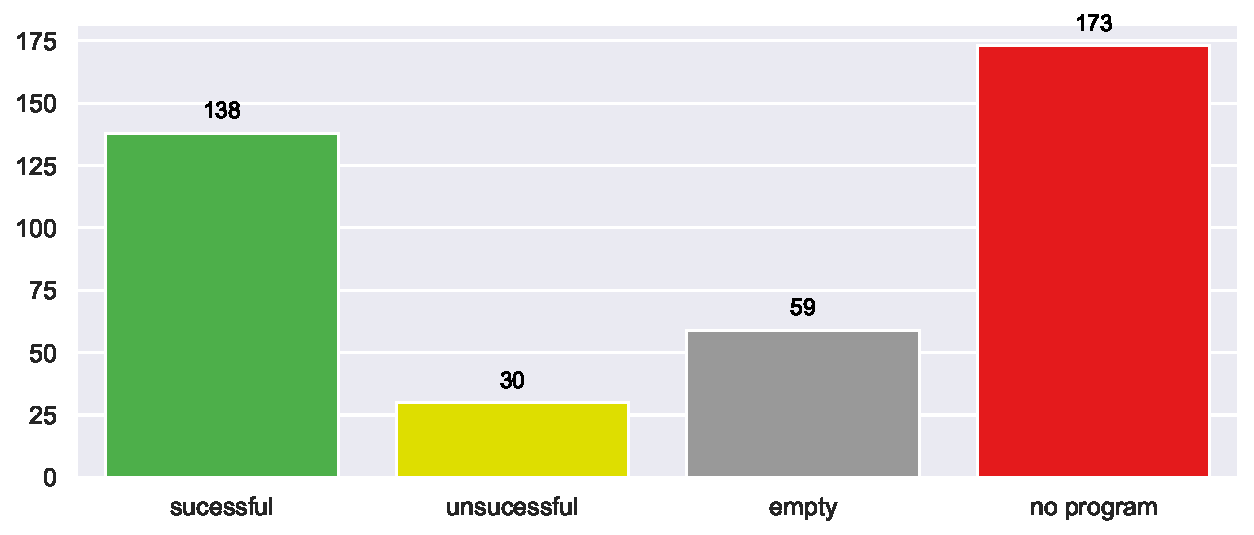
\includegraphics[width=\textwidth, clip]{img/big-study/failure-reason-PBE.pdf}
		\caption{Results of chunk retrieval with PBE}
		\label{fig:failure-reason-PBE}
	\end{minipage}\hfill
	\begin{minipage}{0.45\textwidth}
		\centering
		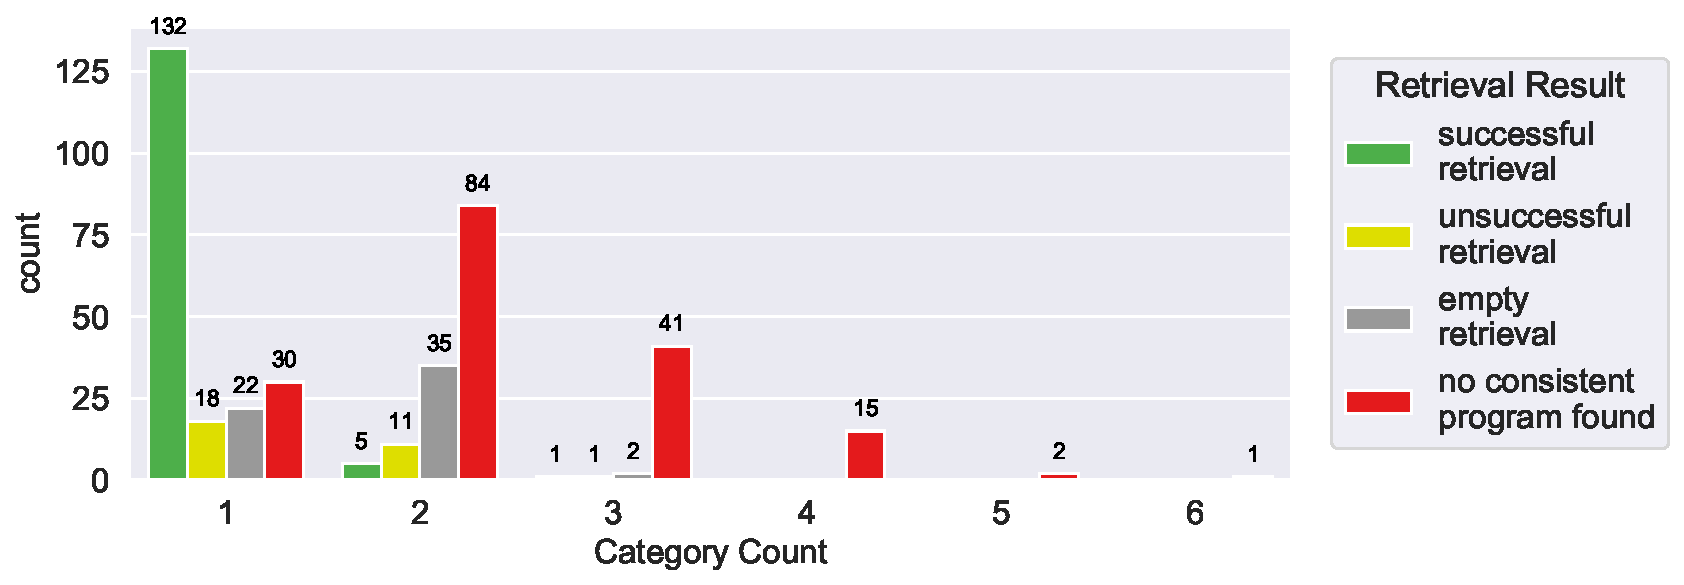
\includegraphics[width=\textwidth, clip]{img/big-study/failure-reason-categorycount-PBE.pdf}
		\caption{Results of chunk retrieval with PBE for numbers of categories present in configuring I/O examples}
		\label{fig:failure-reason-categorycount-PBE}
	\end{minipage}
\end{figure}
\begin{figure}[htbp]
	\centering
	\begin{minipage}{0.45\textwidth}
		\centering
		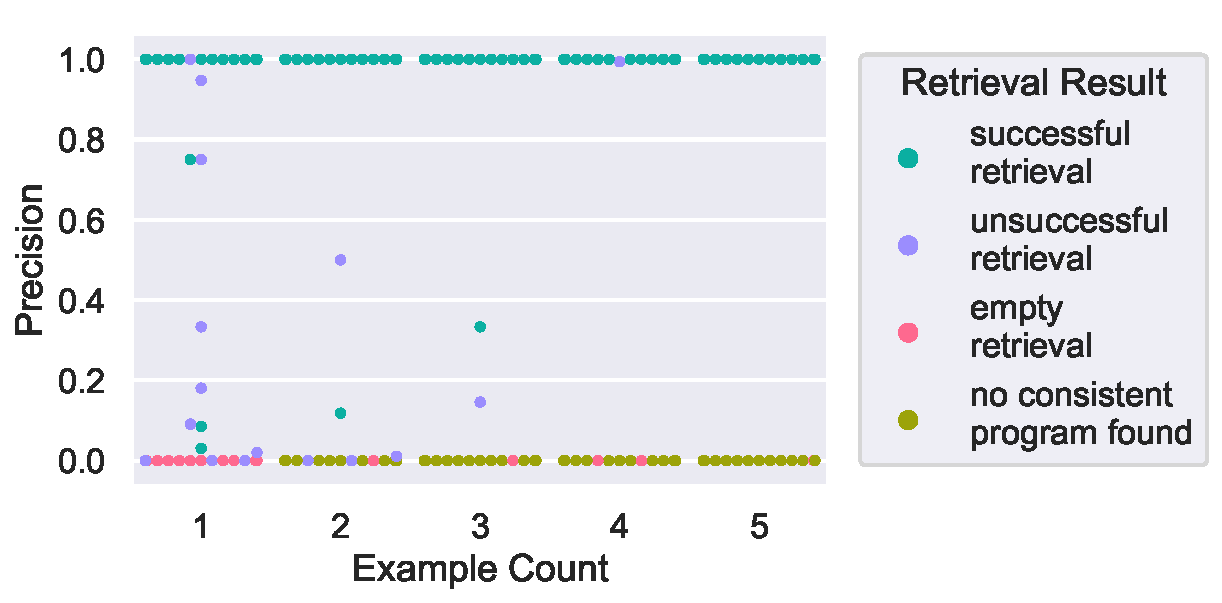
\includegraphics[width=\textwidth, clip]{img/big-study/precision-extraction-result-PBE.pdf}
		\caption{Precision chunk retrieval with PBE for increasing count of configuring I/O examples}
		\label{fig:precision-extraction-result-PBE}
	\end{minipage}\hfill
	\begin{minipage}{0.45\textwidth}
		\centering
		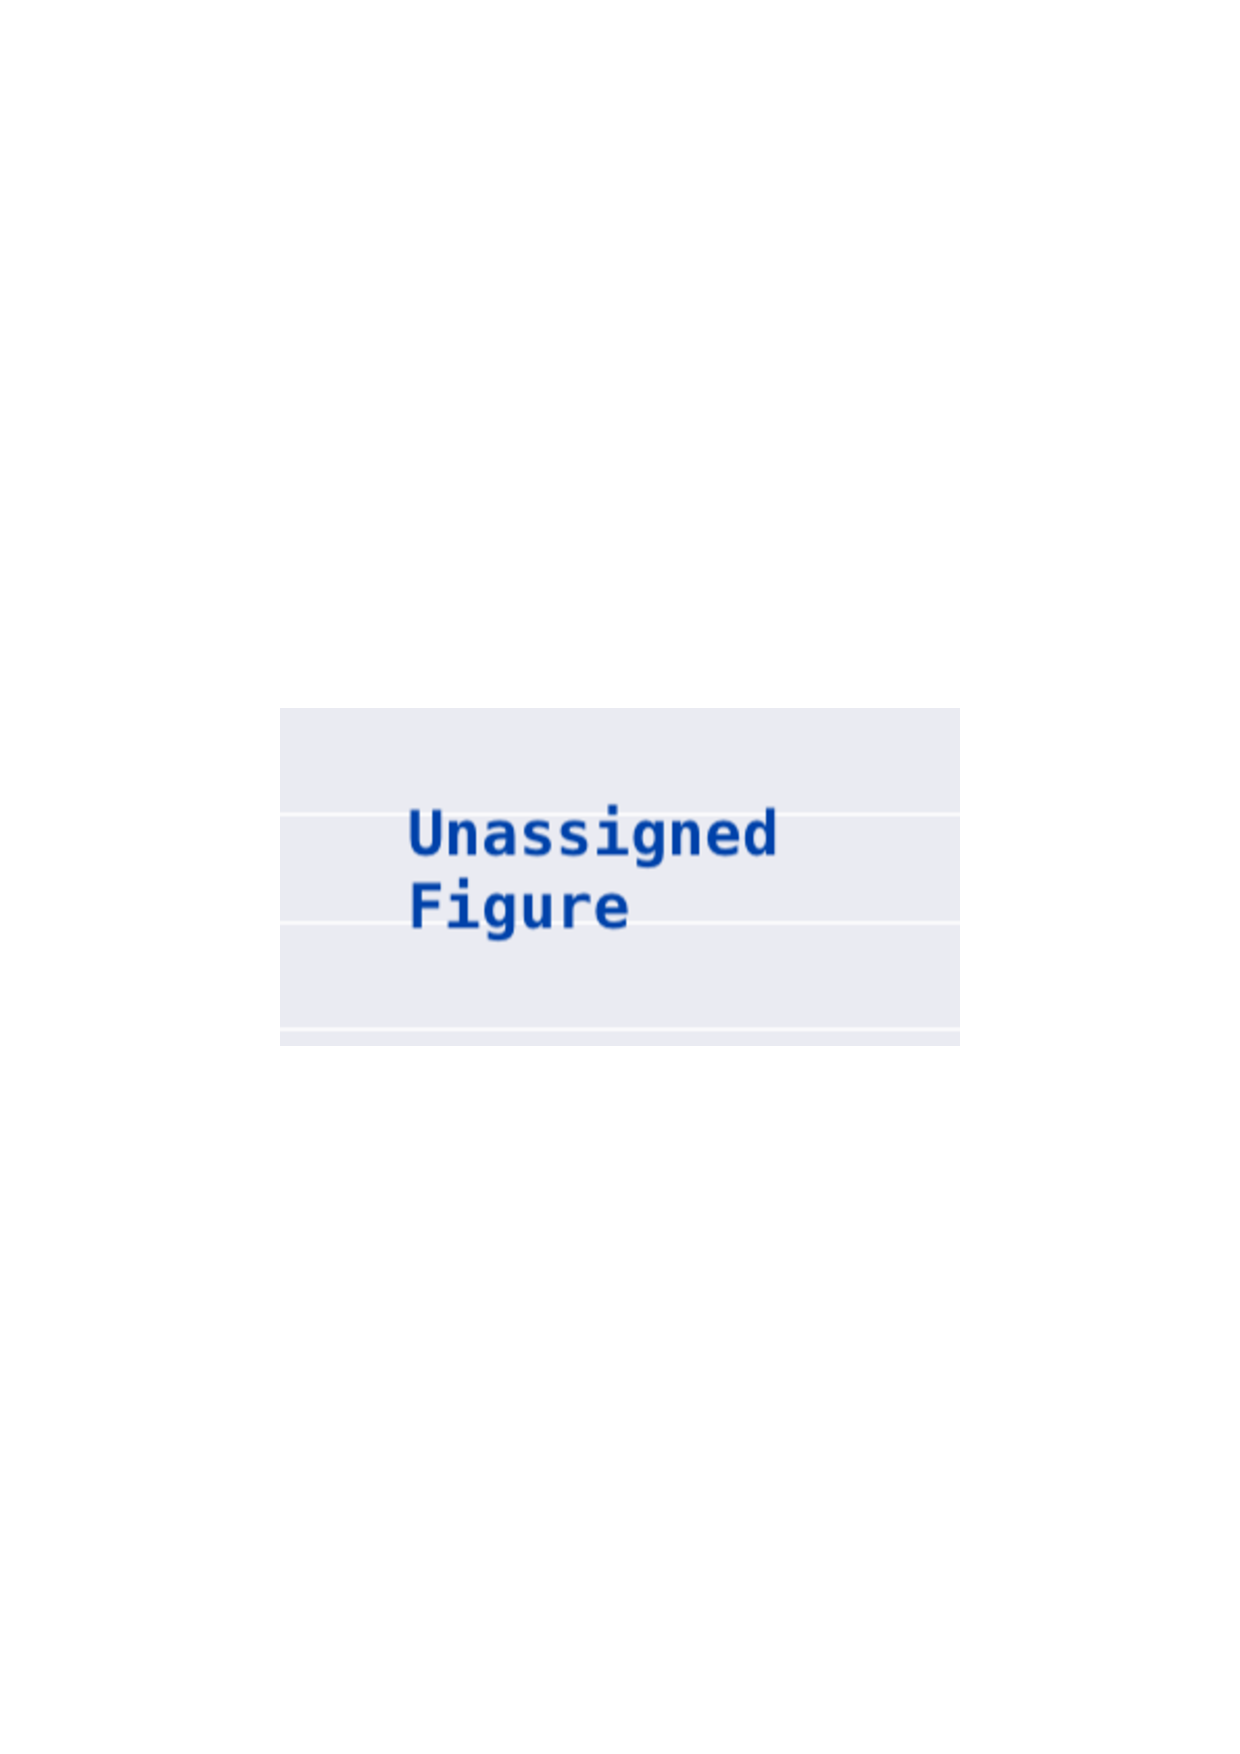
\includegraphics[width=\textwidth, clip]{img/big-study/xxx.pdf}
		\caption{xxx}
		\label{fig:xxx}
	\end{minipage}
\end{figure}
\subsection{Regular Expression Program Synthesis by Example (PBE)}
Figure~\ref{fig:failure-reason-PBE} shows the results of the PBE runs in our evaluation.
Out of the 400 runs, 5 per each one of the 80 example sets, PBE extracted all the desired lines in 138 cases.
Figure \ref{fig:failure-reason-PBE} shows that in 89 further cases a program was also successfully synthesized, though in 59 cases the synthesized program yielded no output at all.
In 30 cases the synthesized program did not extract all of the desired lines, though still had an average recall of 28\%.
In 173 cases the PROSE program synthesis could not synthesize a singular regular expression program that satisfies all of the configuring I/O examples.

Figure \ref{fig:failure-reason-categorycount-PBE} shows the results of PBE runs compared to the number of categories present in the configuring I/O examples.
It shows that the program synthesis is more likely to succeed when there are few categories present in the configuring I/O examples.
When two categories present, PROSE could not synthesize a program consistent with all configuring I/O examples in most cases.
For three or more categories PROSE could never synthesize a consistent program.

Figure \ref{fig:precision-extraction-result-PBE} compares the precision of the PBE chunk retrieval runs with the count of configuring I/O examples.
For one example there is a high number of empty extraction outputs, meaning that the regular expression synthesized from this one I/O example could not be applied to the test I/O example.
For two or more I/O examples the chunk retrieval is either successful or no consistent program could be synthesized.


\begin{figure}[htbp]
	\centering
	\begin{minipage}{0.45\textwidth}
		\centering
		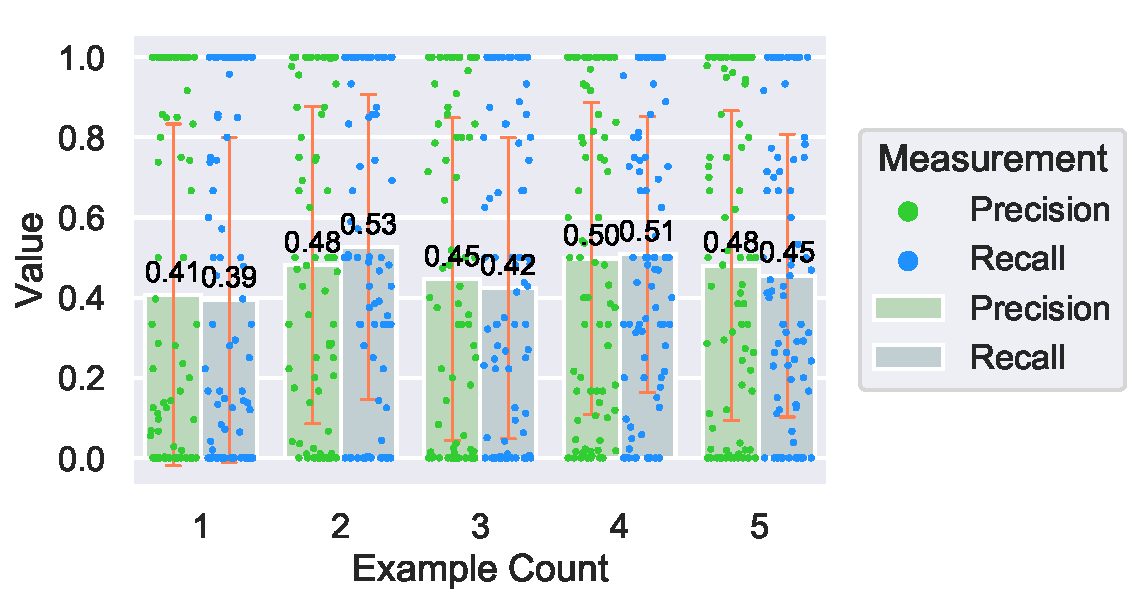
\includegraphics[width=\textwidth, clip]{img/big-study/recall-precision-examplecount-TS.pdf}
		\caption{Paieya}
		\label{fig:recall-precision-examplecount-TS}
	\end{minipage}\hfill
	\begin{minipage}{0.45\textwidth}
		\centering
		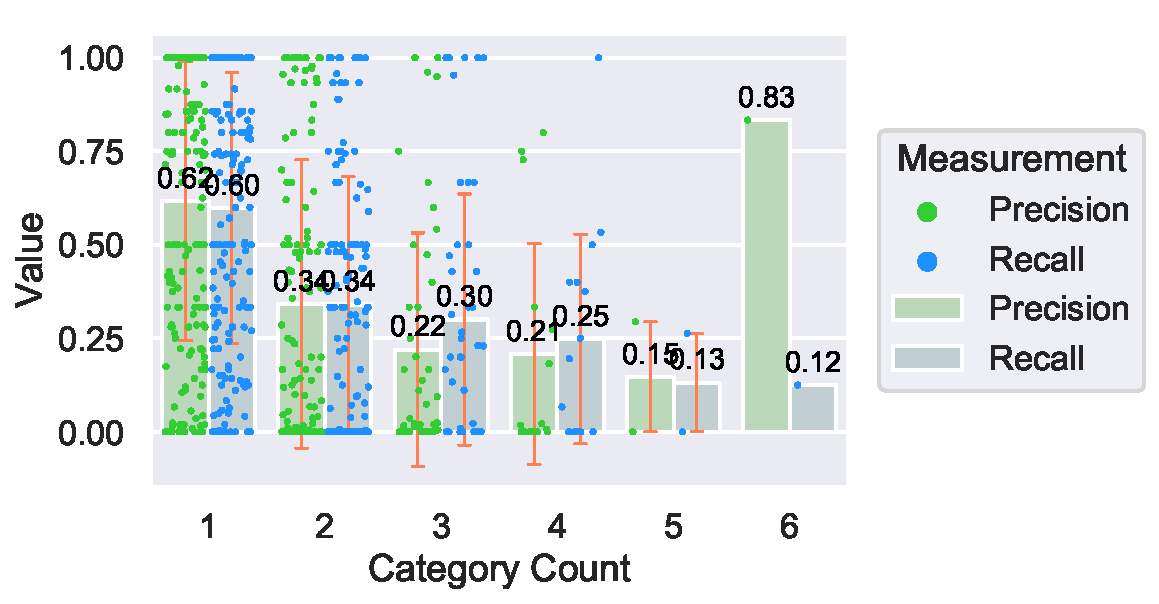
\includegraphics[width=\textwidth, clip]{img/big-study/recall-precision-categorycount-TS.pdf}
		\caption{nei}
		\label{fig:recall-precision-categorycount-TS}
	\end{minipage}
\end{figure}
\begin{figure}[htbp]
	\centering
	\begin{minipage}{0.45\textwidth}
		\centering
		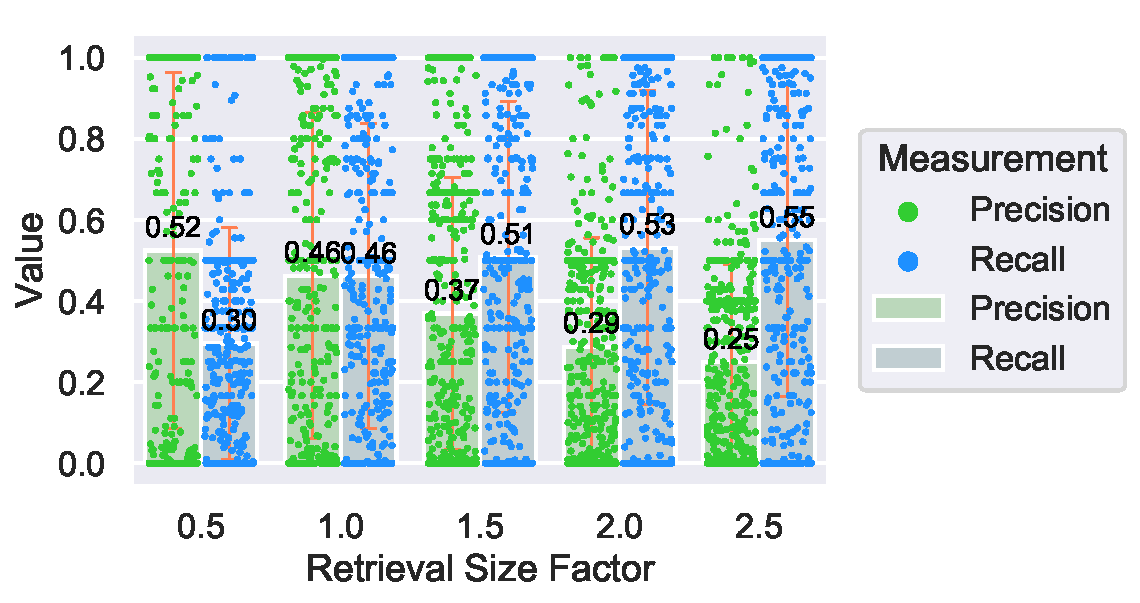
\includegraphics[width=\textwidth, clip]{img/big-study/contextsizefactor-precision-recall-TS.pdf}
		\caption{neind}
		\label{fig:contextsizefactor-precision-recall-TS}
	\end{minipage}\hfill
	\begin{minipage}{0.45\textwidth}
		\centering
		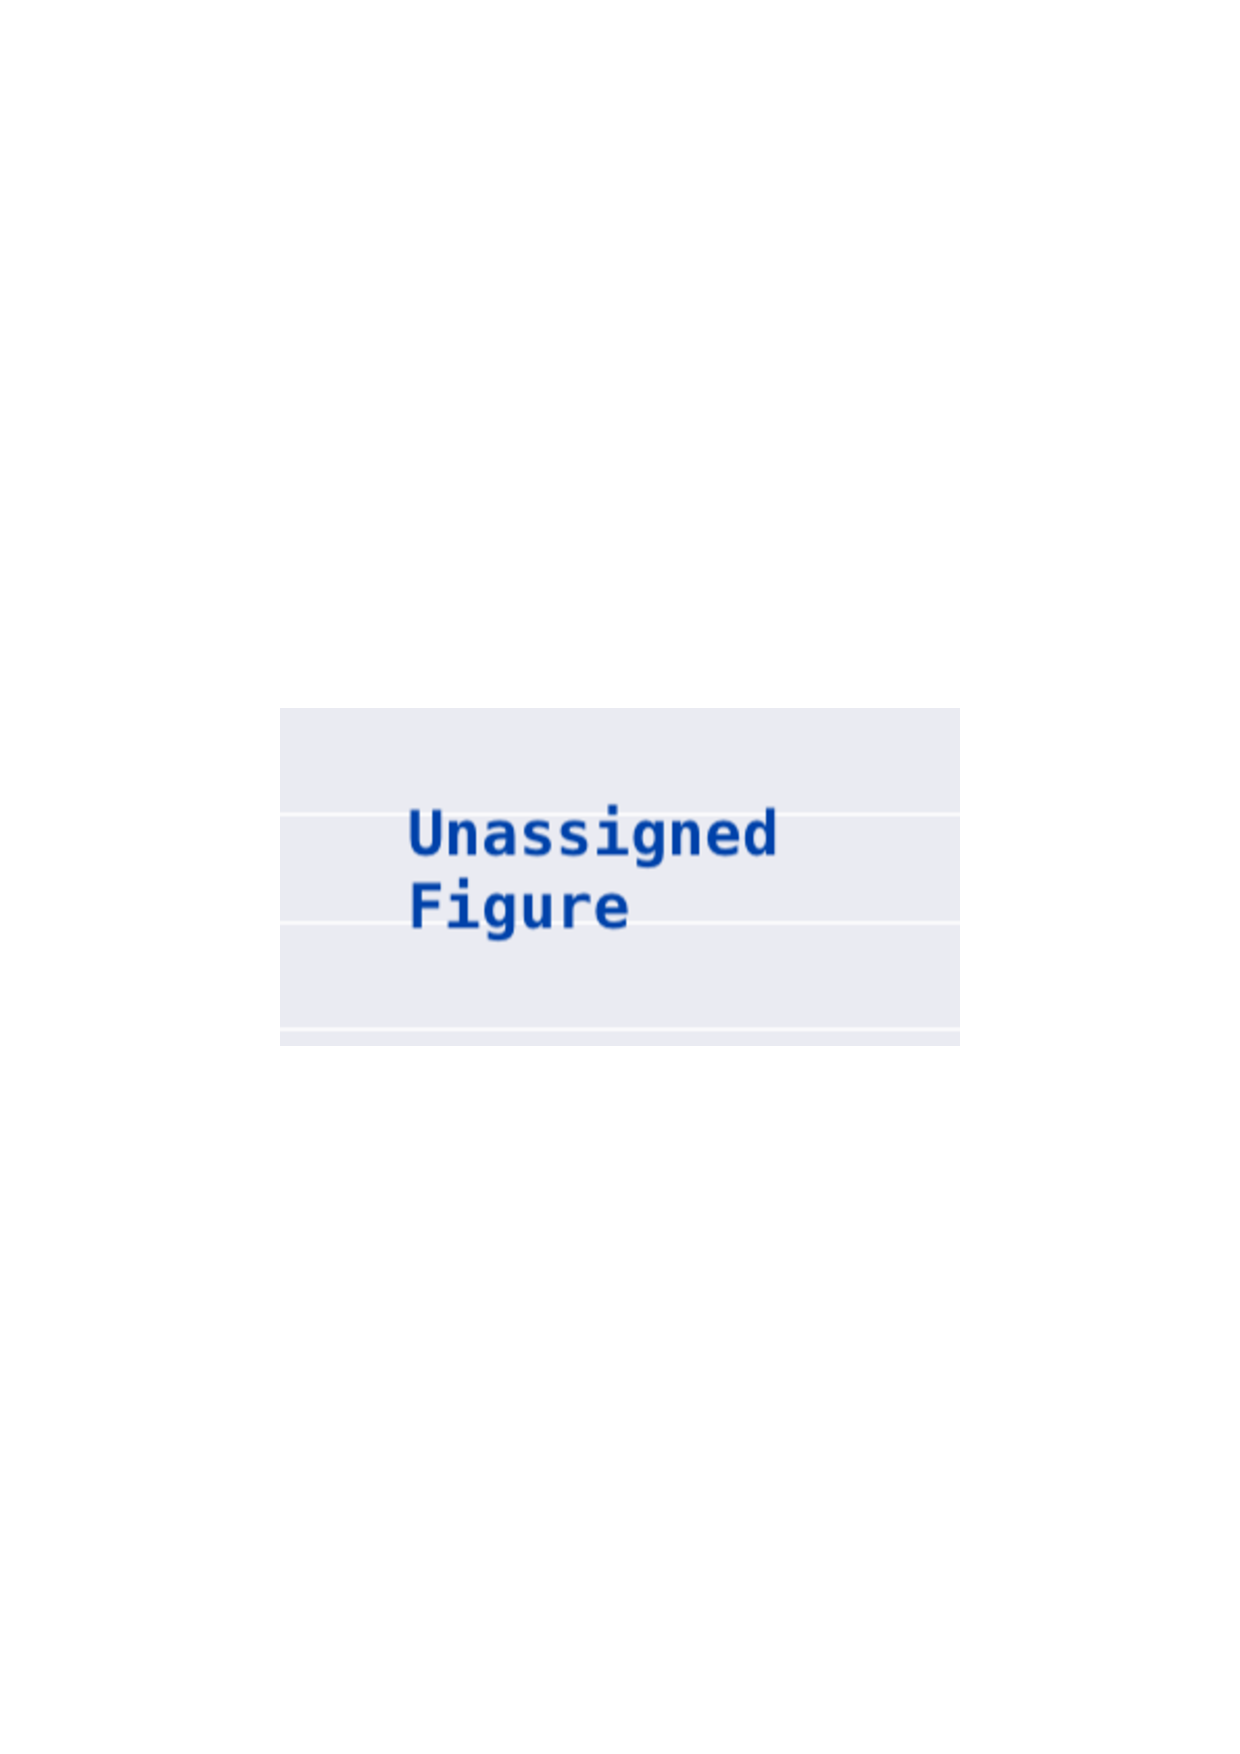
\includegraphics[width=\textwidth, clip]{img/big-study/xxx.pdf}
		\caption{xxx}
		\label{fig:xxx}
	\end{minipage}
\end{figure}

\subsection{Common Text Similarity (CTS)}
Figure \ref{fig:recall-precision-examplecount-TS} presents precision and recall of chunk retrieval using CTS in our study for different numbers of configuring I/O examples.
The count of configuring I/O examples has no visible influence on recall and precision of the chunk retrieval with CTS.

Figure \ref{fig:recall-precision-categorycount-TS} shows the same measurements for different category counts in the configuring I/O examples.
With increasing category count, precision and recall decrease.
Especially for more than three categories present we have no chunk retrieval runs where all desired lines were extracted.

Figure \ref{fig:contextsizefactor-precision-recall-TS} shows the impact of the retrieval size factor on precision and accuracy of chunk retrieval runs with CTS.
The precision ranges from 52\% when retrieving half expected number of lines to 25\% when 2.5 times the expected number of lines.
The recall ranges


% \begin{figure}[htbp]
% 	\centering
% 	\begin{minipage}{0.45\textwidth}
% 		\centering
% 		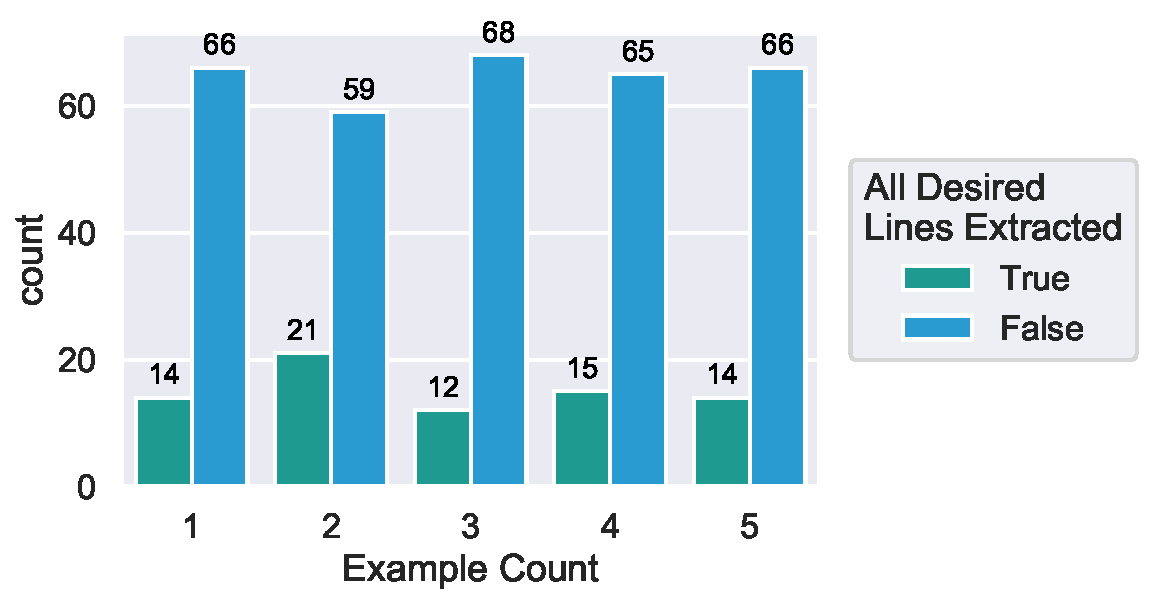
\includegraphics[width=\textwidth, clip]{img/big-study/success-examples-TS.pdf}
% 		\caption{Successful Extractions per Number of Examples for TS}
% 		\label{fig:success-examples-ts}
% 	\end{minipage}\hfill
% 	\begin{minipage}{0.45\textwidth}
% 		\centering
% 		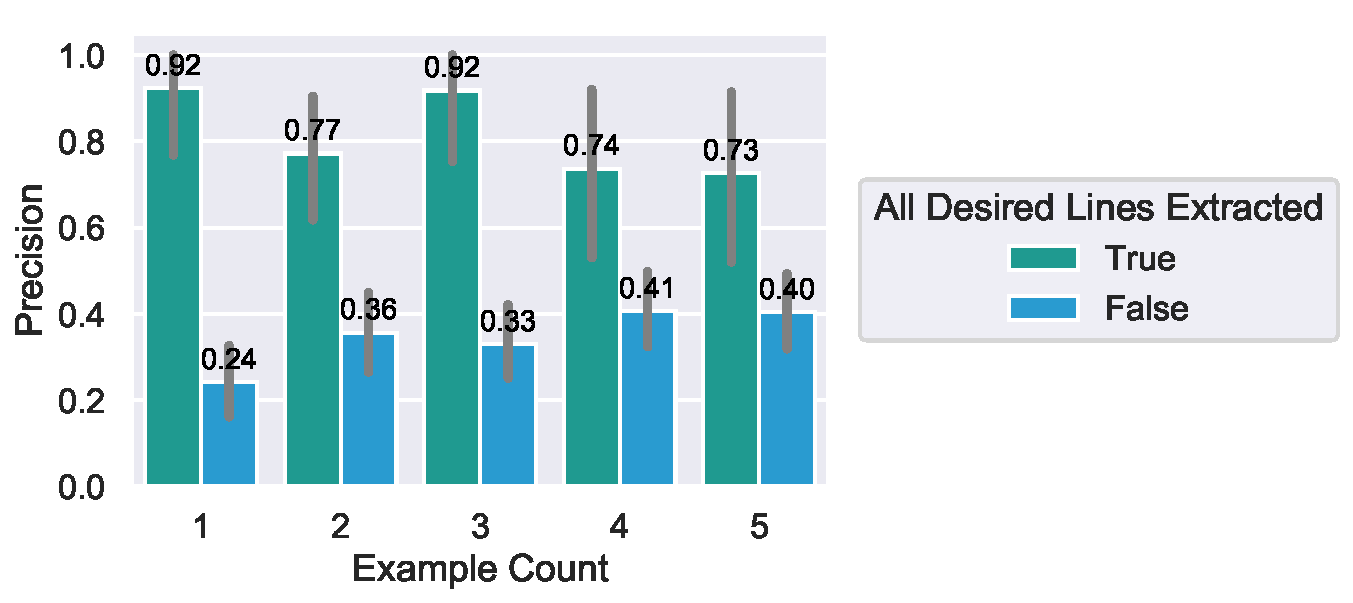
\includegraphics[width=\textwidth, clip]{img/big-study/precision-TS.pdf}
% 		\caption{Precision of Extractions per Number of Examples for TS}
% 		\label{fig:precision-ts}
% 	\end{minipage}
% \end{figure}
% \begin{figure}[htbp]
% 	\centering
% 	\begin{minipage}{0.45\textwidth}
% 		\centering
% 		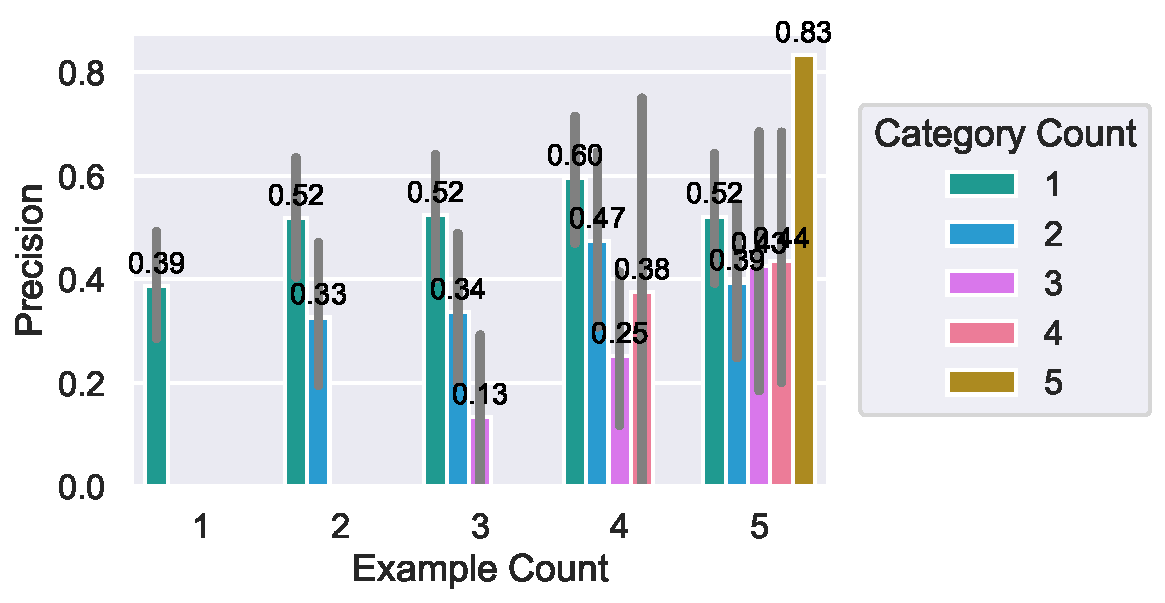
\includegraphics[width=\textwidth, clip]{img/big-study/precision-categorycount-examplecount-TS.pdf}
% 		\caption{Precision of TS Extractions by CategoryCount}
% 		\label{fig:precision-categorycount-examplecount-ts}
% 	\end{minipage}\hfill
% 	\begin{minipage}{0.45\textwidth}
% 		\centering
% 		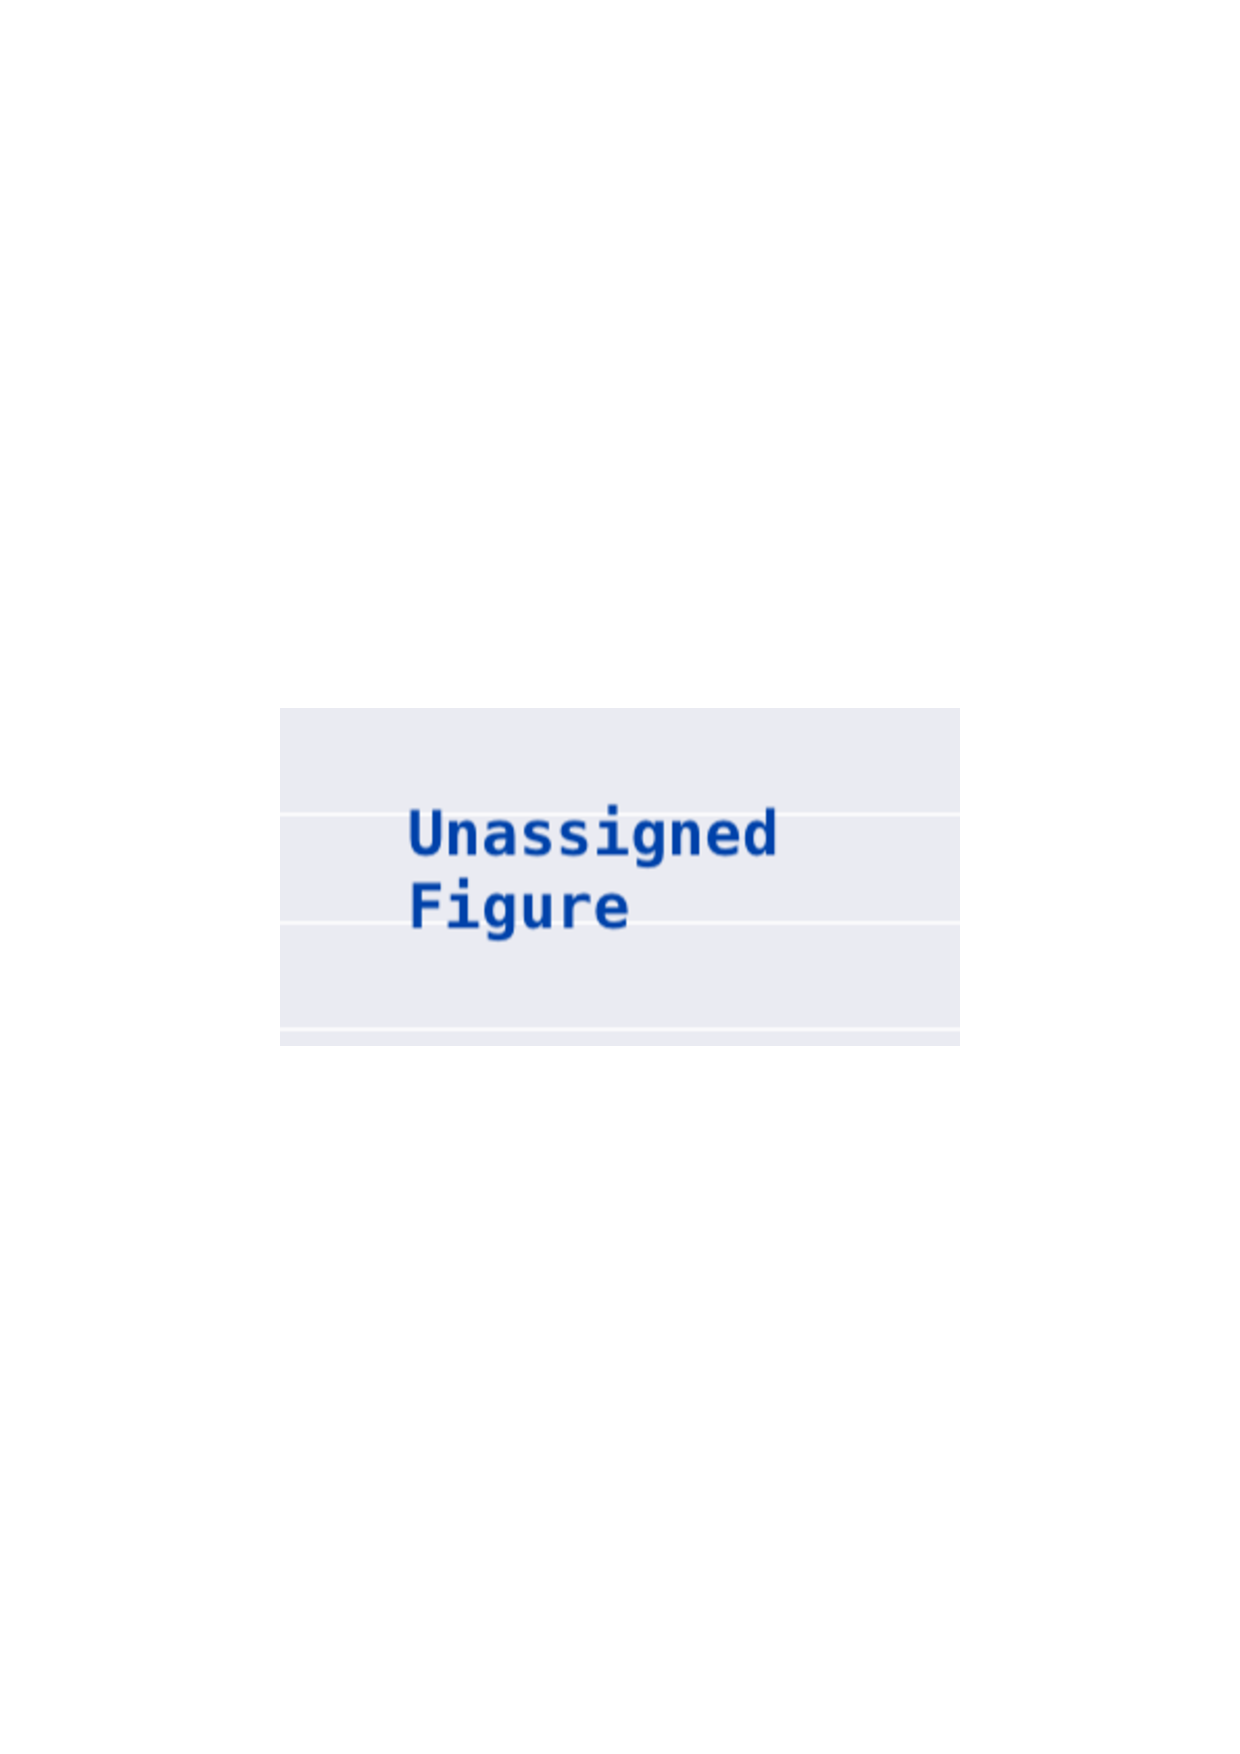
\includegraphics[width=\textwidth, clip]{img/big-study/xxx.pdf}
% 		\caption{xxx}
% 		\label{fig:xxx}
% 	\end{minipage}
% \end{figure}

% \subsubsection{Success-Rate}
% \subsubsection{Precision}
% \subsubsection{Example Categories}


\subsection{Keyword Search (KWS)}

% \begin{figure}[htbp]
% 	\centering
% 	\begin{minipage}{0.45\textwidth}
% 		\centering
% 		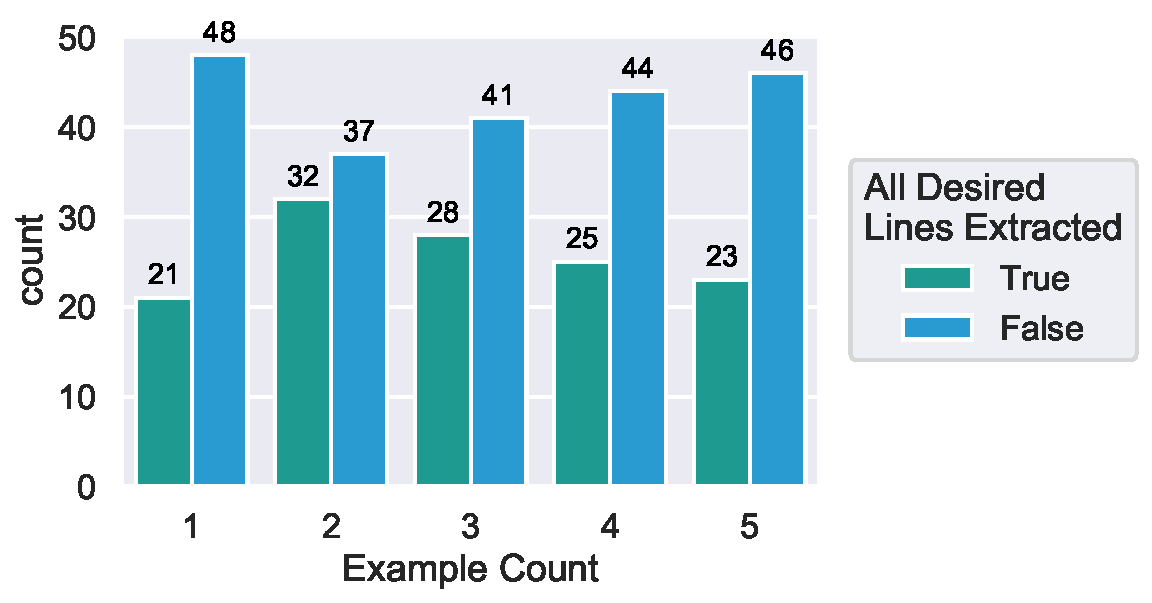
\includegraphics[width=\textwidth, clip]{img/big-study/success-examples-SKWS.pdf}
% 		\caption{Successful Extractions per Number of Examples for SKWS}
% 		\label{fig:success-examples-skws}
% 	\end{minipage}\hfill
% 	\begin{minipage}{0.45\textwidth}
% 		\centering
% 		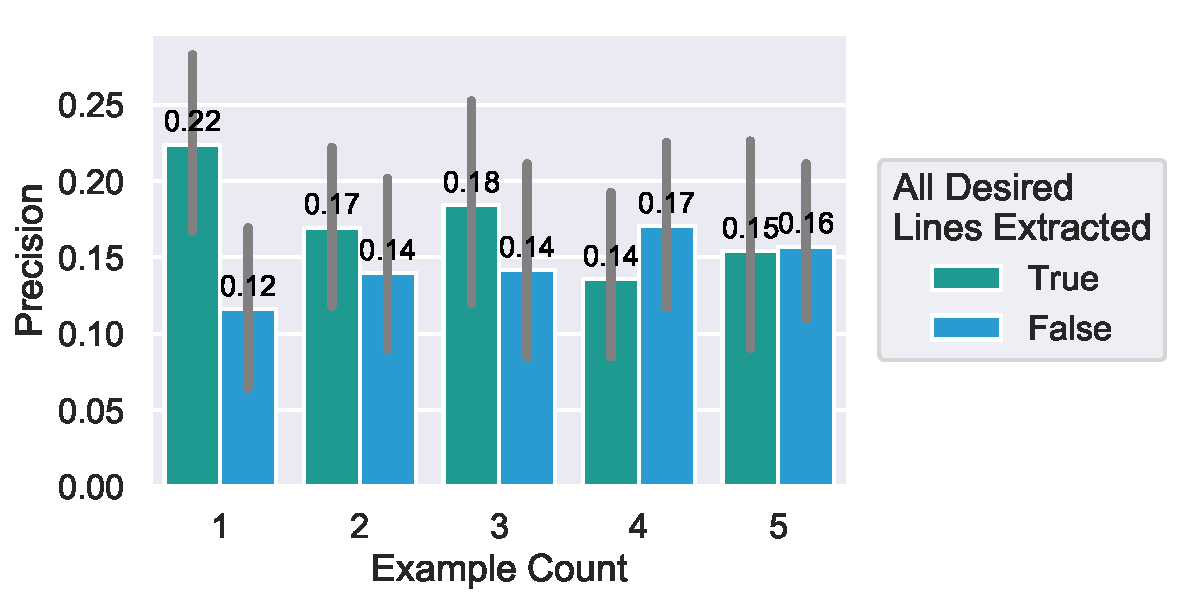
\includegraphics[width=\textwidth, clip]{img/big-study/precision-SKWS.pdf}
% 		\caption{Precision of Extractions per Number of Examples for SKWS}
% 		\label{fig:precision-skws}
% 	\end{minipage}
% \end{figure}
% \begin{figure}[htbp]
% 	\centering
% 	\begin{minipage}{0.45\textwidth}
% 		\centering
% 		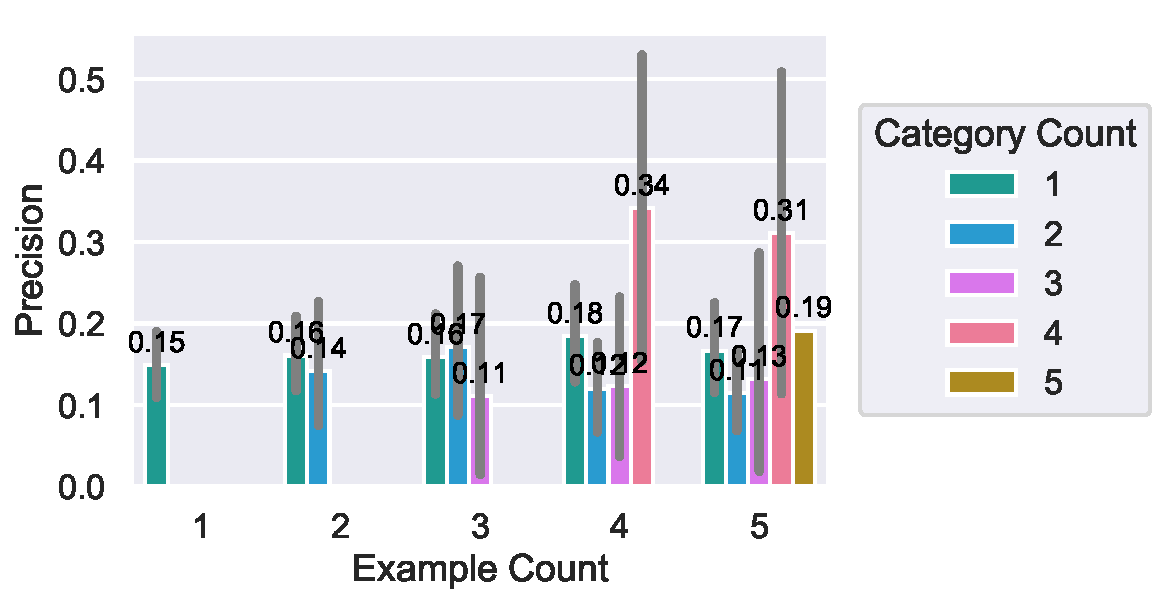
\includegraphics[width=\textwidth, clip]{img/big-study/precision-categorycount-examplecount-SKWS.pdf}
% 		\caption{Precision of SKWS Extractions by CategoryCount}
% 		\label{fig:precision-categorycount-examplecount-skws}
% 	\end{minipage}\hfill
% 	\begin{minipage}{0.45\textwidth}
% 		\centering
% 		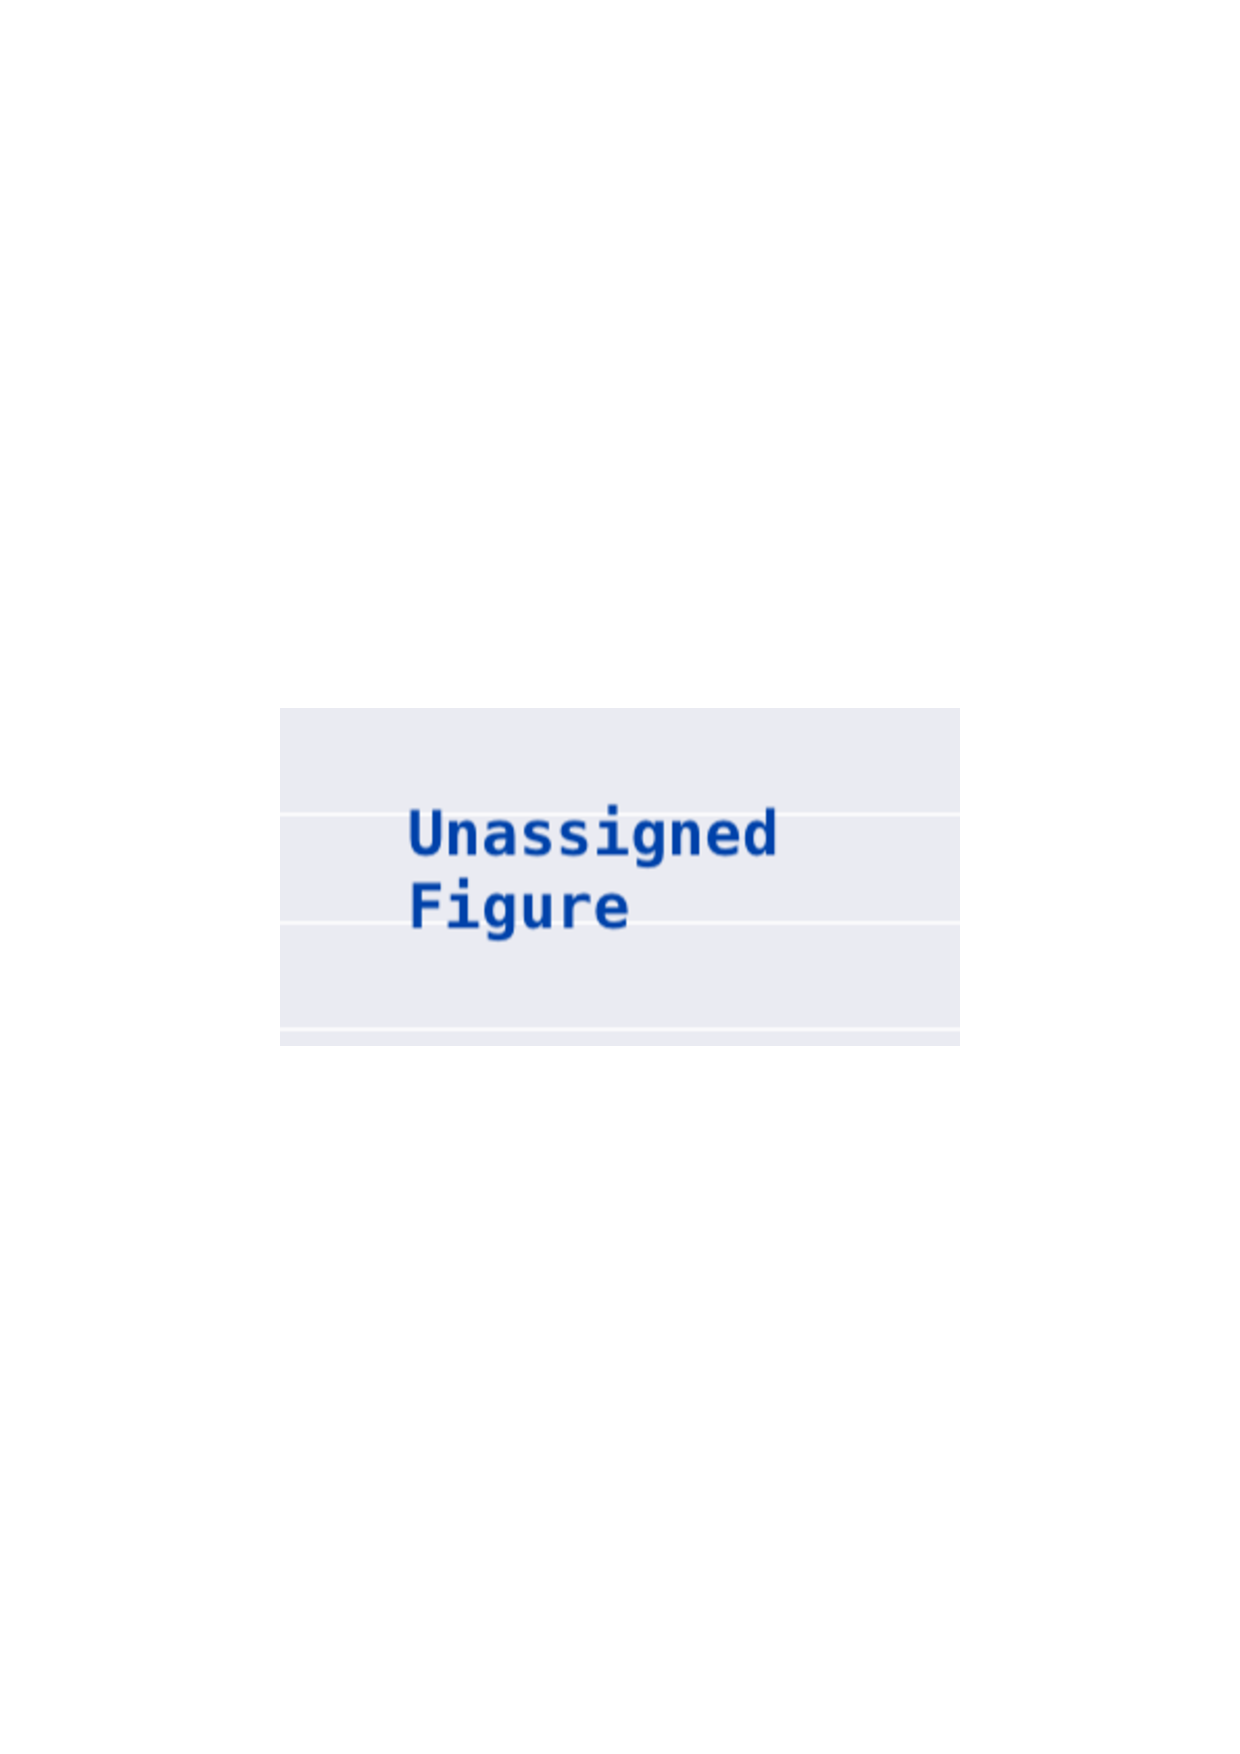
\includegraphics[width=\textwidth, clip]{img/big-study/xxx.pdf}
% 		\caption{xxx}
% 		\label{fig:xxx}
% 	\end{minipage}
% \end{figure}

% \subsubsection{Success-Rate}
% \subsubsection{Precision}
% \subsubsection{Example Categories}


% \subsection{Random Line Retrieval (RLR)}

% \begin{figure}[htbp]
% 	\centering
% 	\begin{minipage}{0.45\textwidth}
% 		\centering
% 		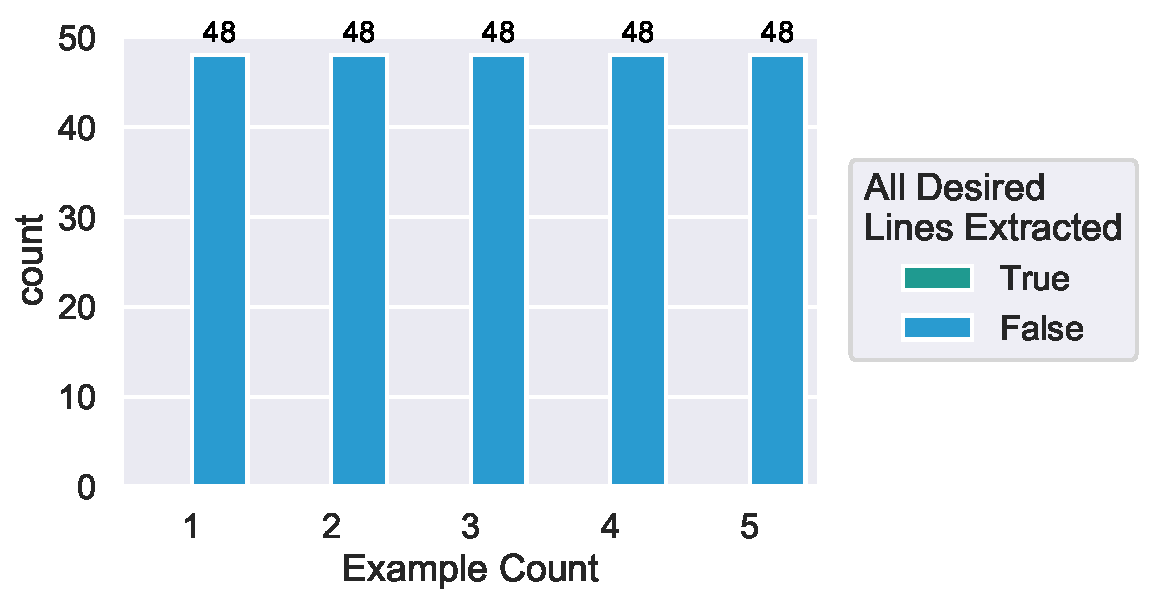
\includegraphics[width=\textwidth, clip]{img/big-study/success-examples-RLR.pdf}
% 		\caption{Successful Extractions per Number of Examples for RLR}
% 		\label{fig:success-examples-rlr}
% 	\end{minipage}\hfill
% 	\begin{minipage}{0.45\textwidth}
% 		\centering
% 		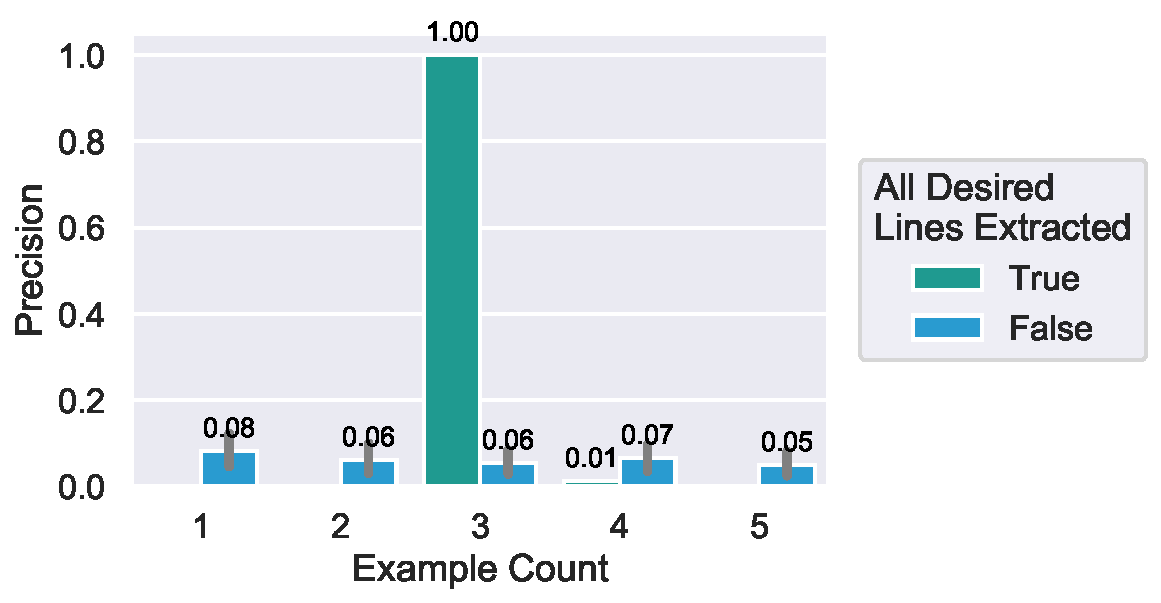
\includegraphics[width=\textwidth, clip]{img/big-study/precision-RLR.pdf}
% 		\caption{Precision of Extractions per Number of Examples for RLR}
% 		\label{fig:precision-rlr}
% 	\end{minipage}
% \end{figure}
% \begin{figure}[htbp]
% 	\centering
% 	\begin{minipage}{0.45\textwidth}
% 		\centering
% 		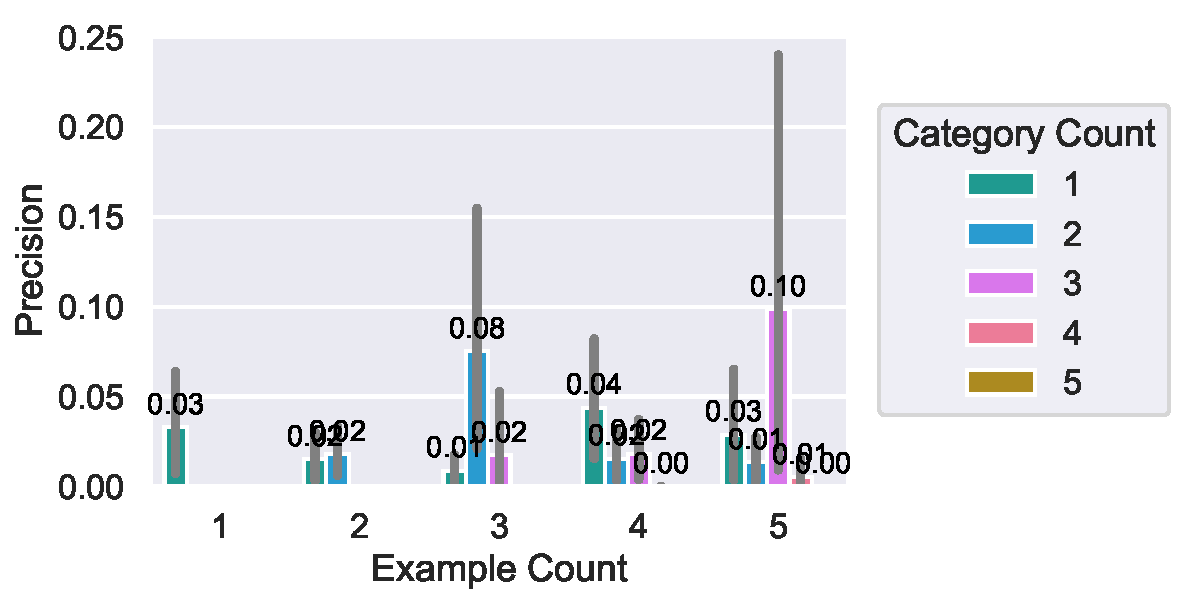
\includegraphics[width=\textwidth, clip]{img/big-study/precision-categorycount-examplecount-RLR.pdf}
% 		\caption{Precision of RLR Extractions by CategoryCount}
% 		\label{fig:precision-categorycount-examplecount-rlr}
% 	\end{minipage}\hfill
% 	\begin{minipage}{0.45\textwidth}
% 		\centering
% 		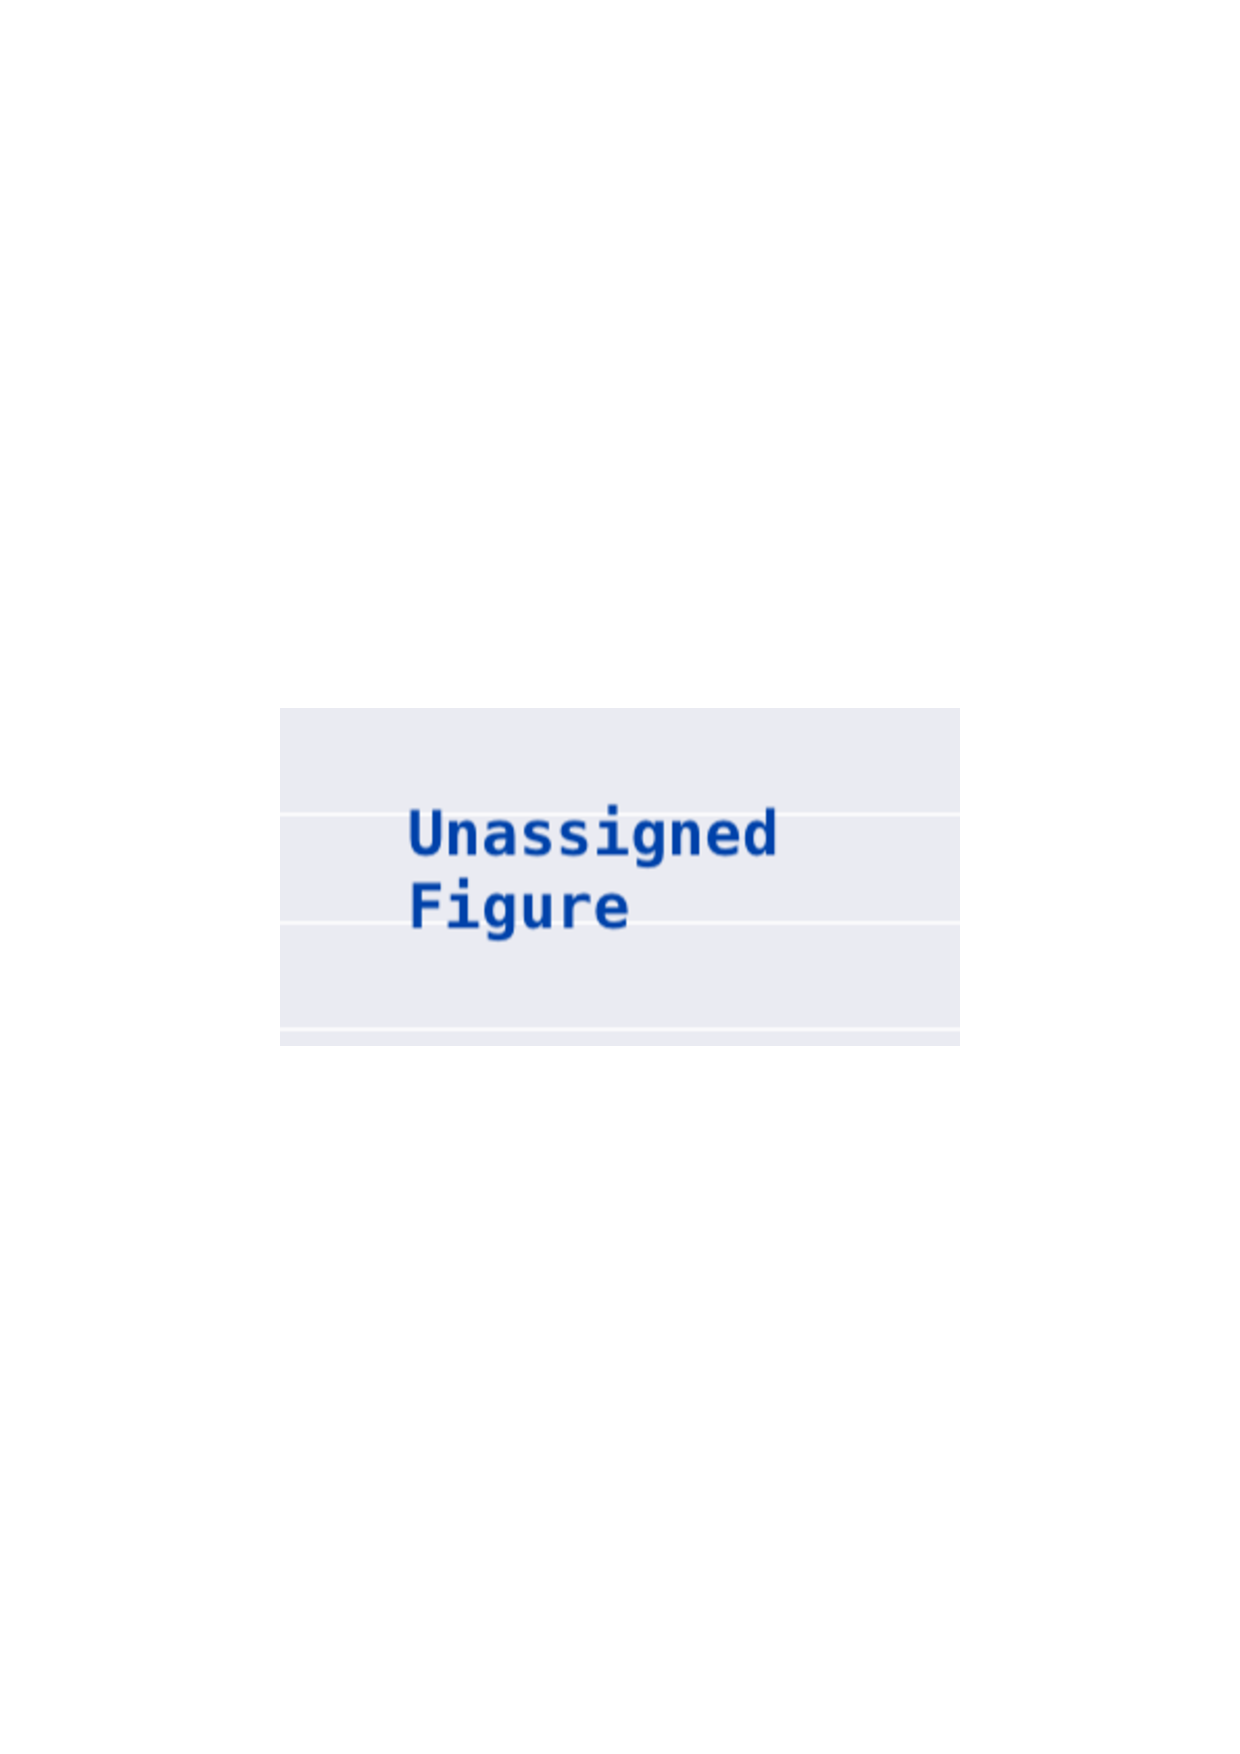
\includegraphics[width=\textwidth, clip]{img/big-study/xxx.pdf}
% 		\caption{xxx}
% 		\label{fig:xxx}
% 	\end{minipage}
% \end{figure}

% For completion this section reports the results for the random line retrieval technique, explained in detail in Section \ref{sec:}

% \subsubsection{Success-Rate}
% \subsubsection{Precision}
% \subsubsection{Example Categories}

\subsection{Comparing All Techniques}
% \begin{figure}[htbp]
% 	\centering
% 	\begin{minipage}{0.45\textwidth}
% 		\centering
% 		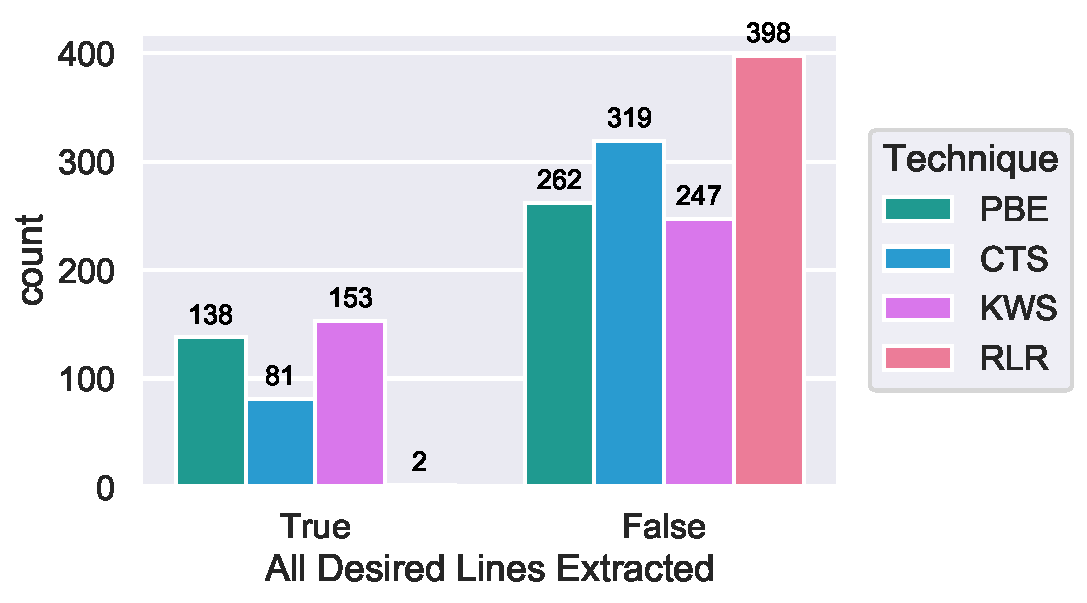
\includegraphics[width=\textwidth, clip]{img/big-study/success-all.pdf}
% 		\caption{Successful Extractions for all Techniques Compared}
% 		\label{fig:success-all}
% 	\end{minipage}\hfill
% 	\begin{minipage}{0.45\textwidth}
% 		\centering
% 		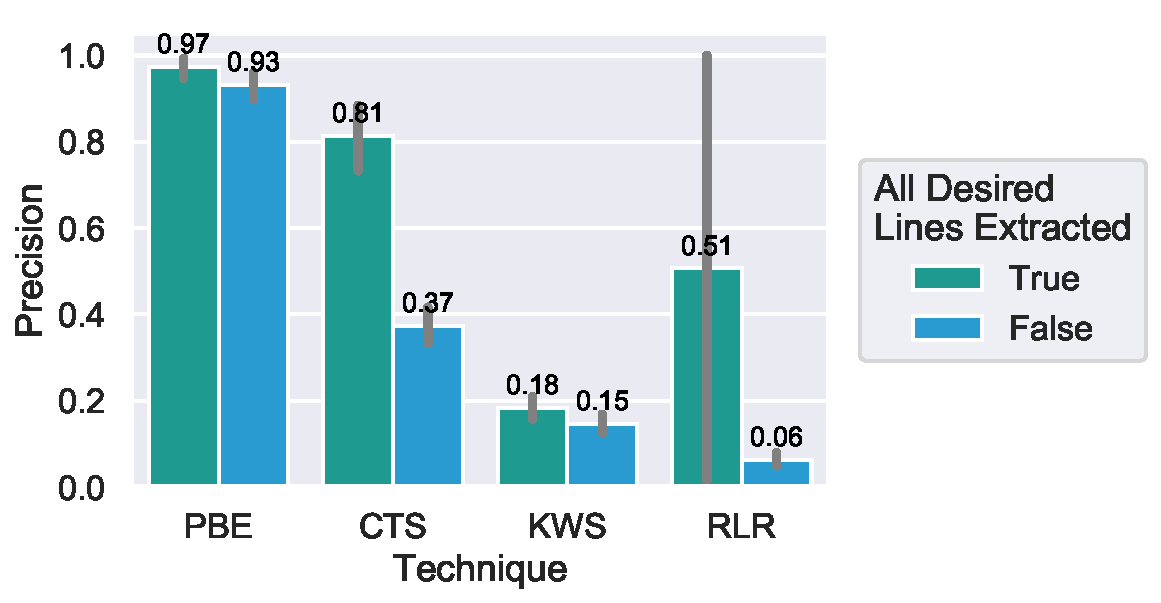
\includegraphics[width=\textwidth, clip]{img/big-study/precision-all.pdf}
% 		\caption{Precision of Extractions for all Techniques Compared}
% 		\label{fig:precision-all}
% 	\end{minipage}
% \end{figure}

% \begin{figure}[htbp]
% 	\centering
% 	\begin{minipage}{0.45\textwidth}
% 		\centering
% 		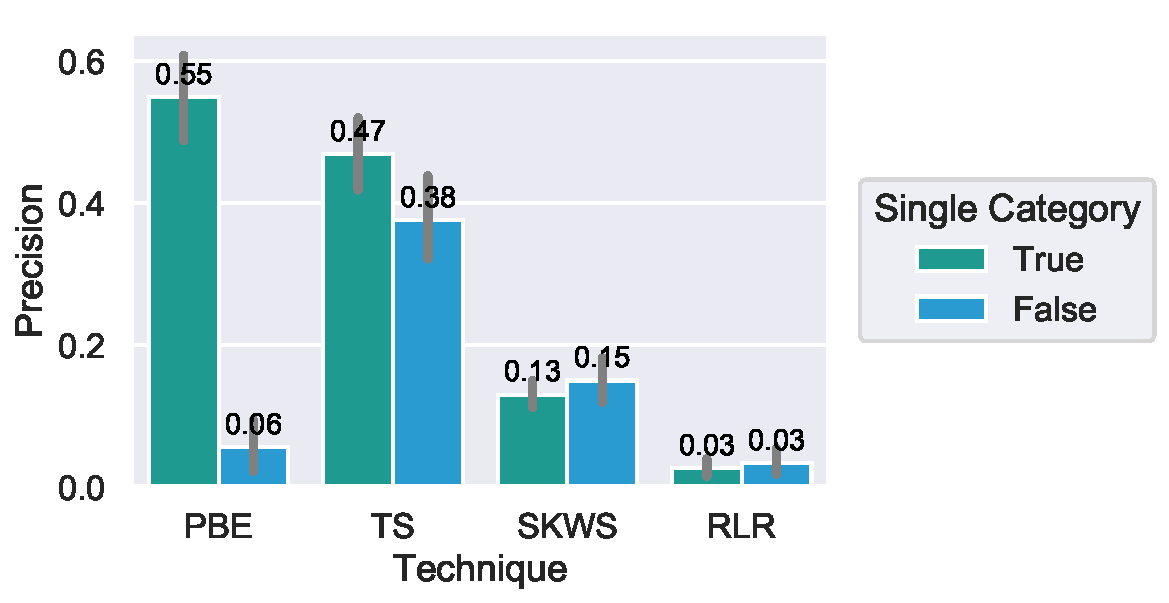
\includegraphics[width=\textwidth, clip]{img/big-study/precision-category-singularity-all.pdf}
% 		\caption{\todo{todo}}
% 		\label{fig:precision-category-singularity-all}
% 	\end{minipage}\hfill
% 	\begin{minipage}{0.45\textwidth}
% 		\centering
% 		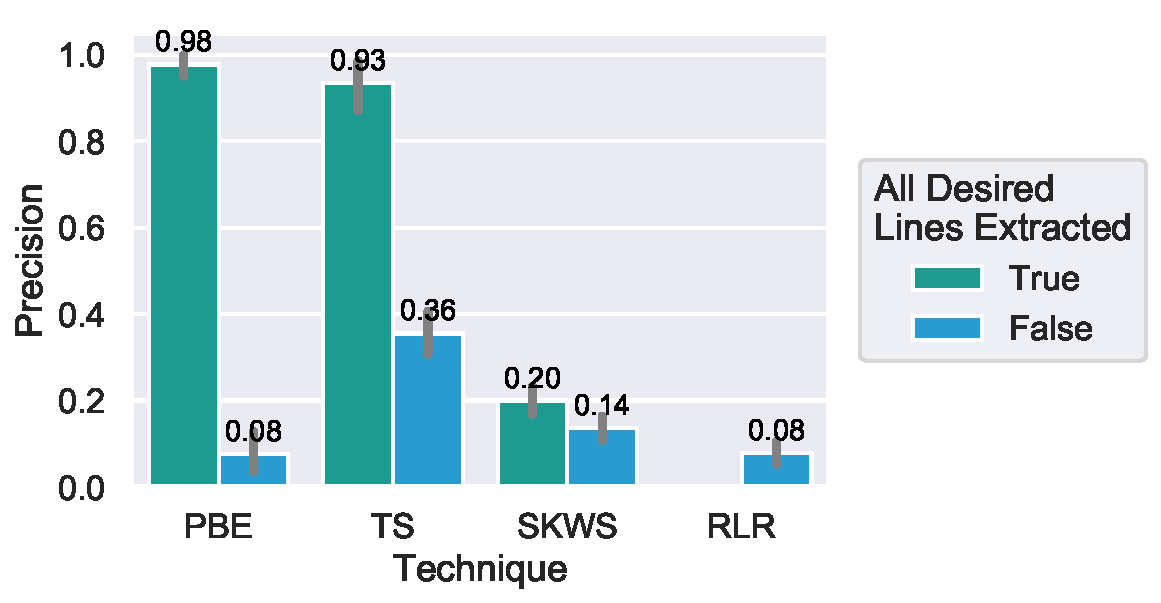
\includegraphics[width=\textwidth, clip]{img/big-study/single-cateogry-precision-all.pdf}
% 		\caption{\todo{todo}}
% 		\label{fig:single-cateogry-precision-all}
% 	\end{minipage}
% \end{figure}

% \begin{figure}[htbp]
% 	\centering
% 	\begin{minipage}{0.45\textwidth}
% 		\centering
% 		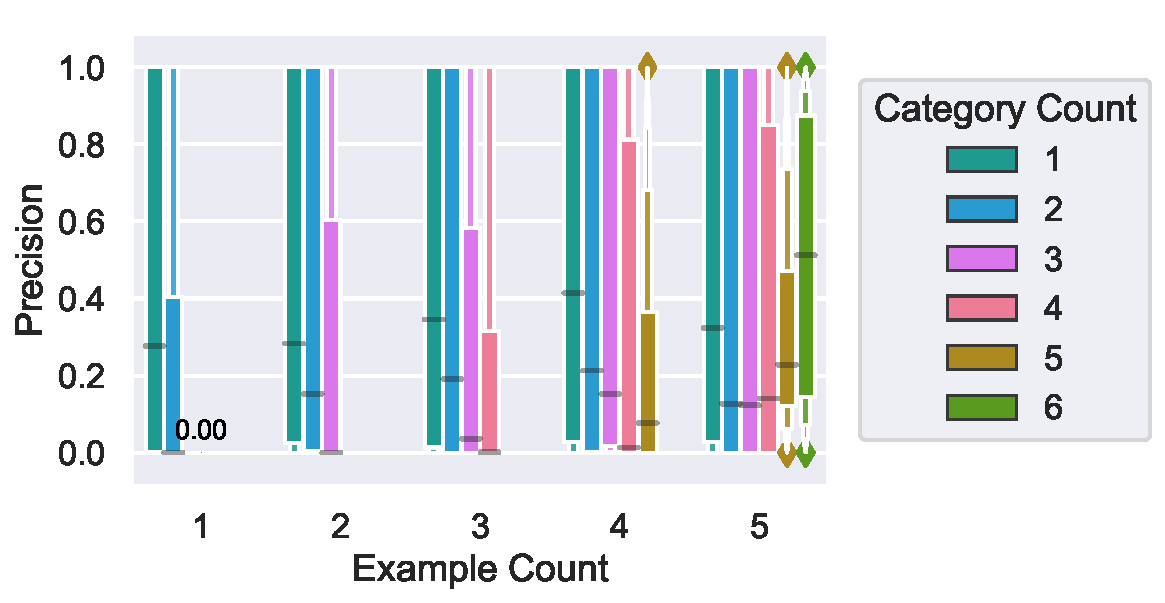
\includegraphics[width=\textwidth, clip]{img/big-study/precision-categorycount-examplecount-all.pdf}
% 		\caption{\todo{todo}}
% 		\label{fig:precision-categorycount-examplecount-all}
% 	\end{minipage}\hfill
% 	\begin{minipage}{0.45\textwidth}
% 		\centering
% 		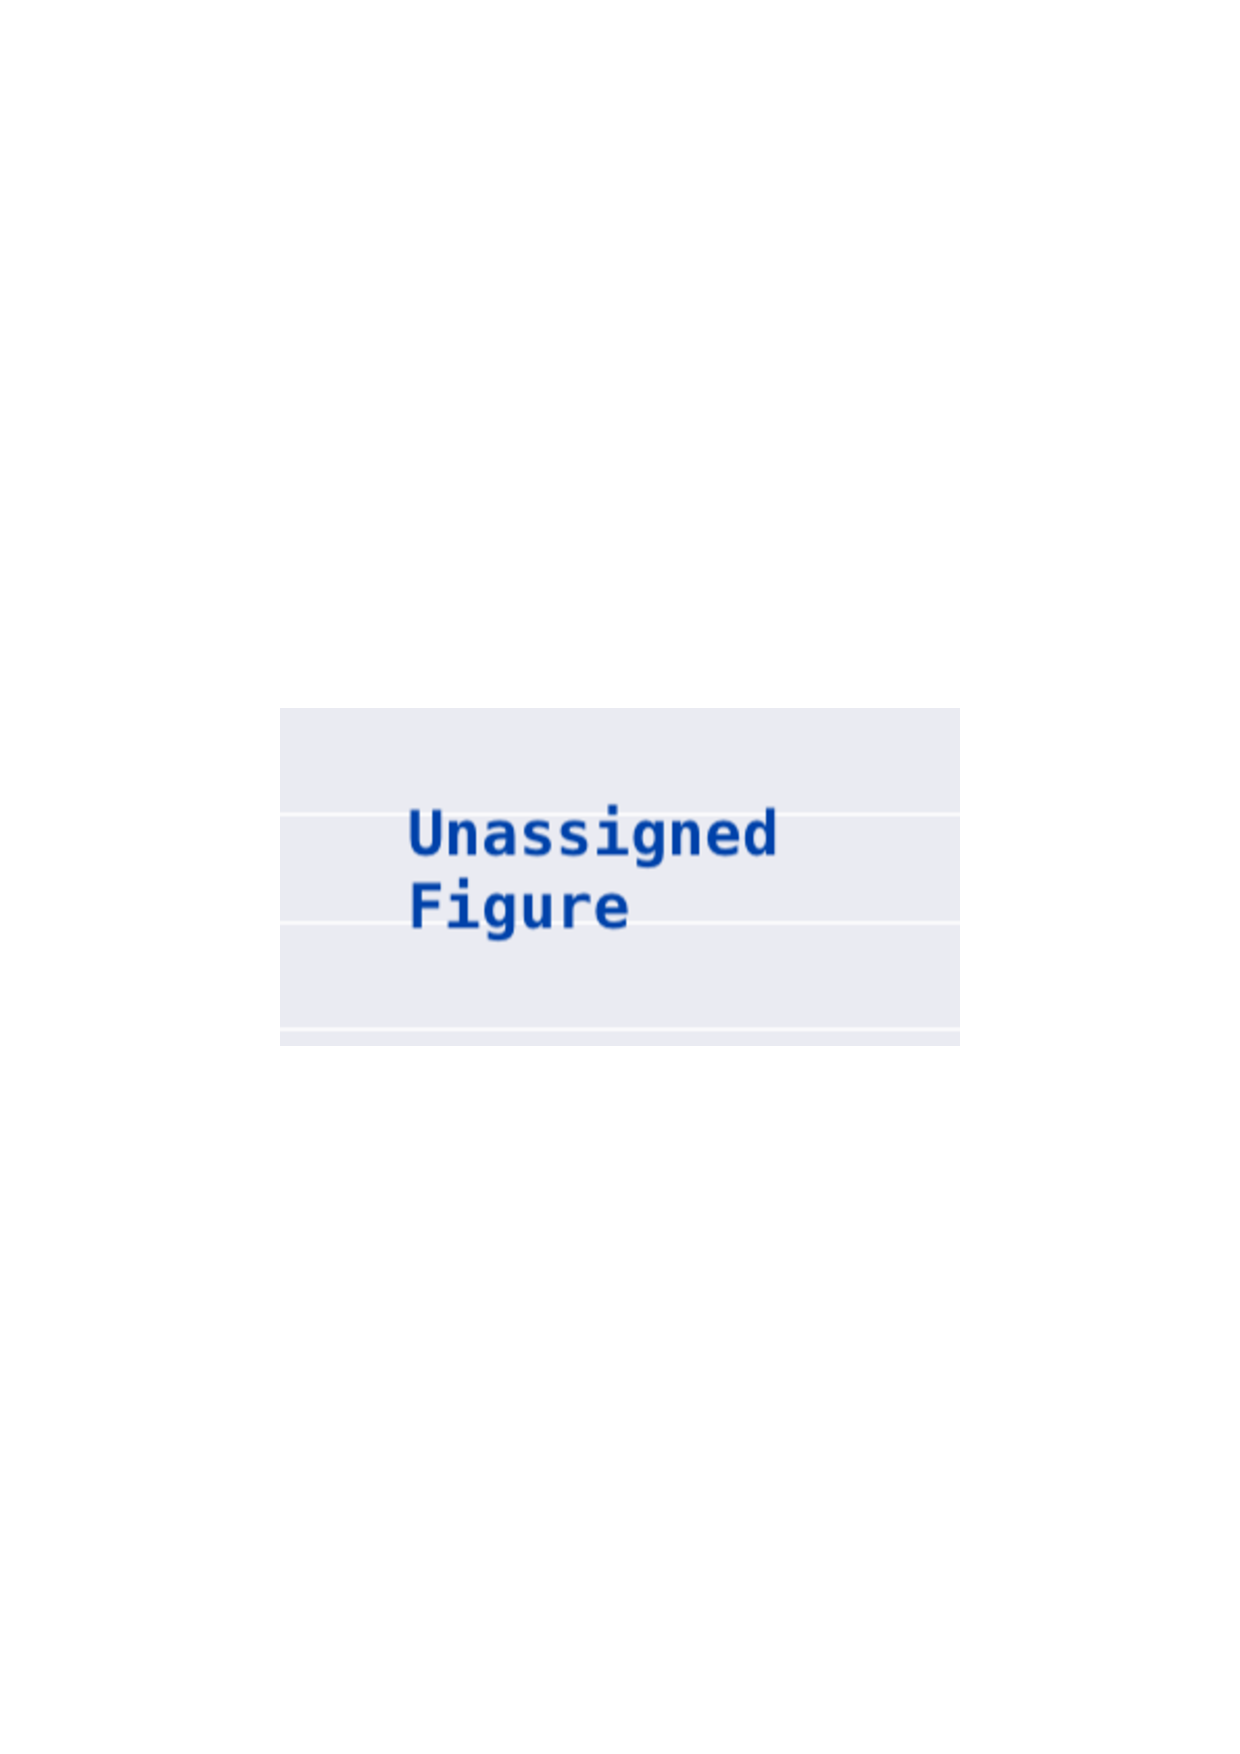
\includegraphics[width=\textwidth, clip]{img/big-study/xxx.pdf}
% 		\caption{\todo{todo}}
% 		\label{fig:xxx}
% 	\end{minipage}
% \end{figure}

% \subsubsection{Success-Rate}
% \subsubsection{Precision}
% \subsubsection{Example Categories}

% \section{Discussion}
% \todo{draw decision tree}

% interpret results - when should PROSE be used? - when should text similarity be used? - when should keyword search be used? - answer RQ about PROSE \& other techniques
\section{Threats to Validity}
%chronologically selected examples -> very specific view



\end{document}
